\documentclass[aspectratio=169,xcolor=dvipsnames, 11pt,mathserif]{beamer} 
% \documentclass[aspectratio=169,xcolor=dvipsnames, 11pt,mathserif]{beamer} 
% Put this line above % \documentclass[aspectratio=169,xcolor=dvipsnames, 11pt,mathserif]{beamer} 
% Put this line above % \documentclass[aspectratio=169,xcolor=dvipsnames, 11pt,mathserif]{beamer} 
% Put this line above \input{preamble_slides.tex} otherwise it may cause bug

%\documentclass[xcolor=dvipsnames,mathserif]{beamer} % this option has curvier math
%\documentclass[xcolor=dvipsnames,11pt]{beamer}
% Note: the color structure needs to be added here in the title. Now it recognizes all beamer % colors.

%%%%%%%%  PRESENTATION LAYOUT:
\usepackage{appendixnumberbeamer} % this package does not count the appendix pages. /!\ Inconstant behavior, sometimes bug.
\mode<presentation>
{
  \usetheme{Boadilla}
  \usecolortheme{lily} % lily is nice or orchid but not for definition
  \setbeamercovered{invisible}
  \setbeamertemplate{footline}{\raggedleft\insertframenumber~/~\inserttotalframenumber\hspace*{3pt}\vskip3pt} %this command shows frame number, not page number at bottom (means if using overlays, % frame number does not change)
%\setbeamertemplate{footline}[page number]  % this puts only page number on bottom
 \setbeamertemplate{navigation symbols}{t}  % this erases navigation symbols.
 \setbeamersize{text margin left=0.1cm, text margin right=0.1cm} % left=0.2cm
 \setbeamertemplate{frametitle}[default][center]
 \setbeamercolor{frametitle}{fg=black}
 \setbeamerfont{frametitle}{size=\large, series=\bfseries} % Modifies frame title font.
 \setbeamercolor{button}{fg=blue, bg=white}
 \setbeamertemplate{itemize item}[circle]
 \setbeamercolor{itemize item}{fg=black}
 \setbeamercolor{itemize/enumerate body}{fg=black}
 \setbeamerfont{framesubtitle}{series=\mdseries}
}

\renewcommand{\familydefault}{\rmdefault} %Options here are \ttdefault \ssdefault or \rmdefault.

% This defines actual color palette; 
\definecolor{blue}{RGB}{0,114,178}
\definecolor{orangered}{RGB}{213,94,0}
\definecolor{yellow}{RGB}{240,228,66}
\definecolor{green}{RGB}{0,158,115}
\definecolor{orange}{RGB}{230,159,0}

\hypersetup{
  colorlinks = false,
  linkbordercolor = {white},
  linkcolor = {blue}
}

%%% Color customization: where these colors are used. 
\colorlet{cwords}{blue} %this defines a color, stored under the name cwords that will be used and recognized in document.
\colorlet{cwordsc}{red} %color for contrast with some other word.
\colorlet{cwords2}{green} %2nd color for contrast with some other word.
\colorlet{cmath}{blue} %color for math in text.
%\everymath{\color{blue}} % This in conjunction with the everysel package sets color of math
\everydisplay{\color{blue}}


%%%%%%%%  PACKAGES USED:
\usepackage{amsmath}
\usepackage{setspace} % Only needed for spacing
\usepackage{changepage} % Only needed for local margin setting
\usepackage{mathpazo}% font, is overwritten by times
%\usepackage[hypertexnames=false]{hyperref} %This makes hyperref ``dumber'', and, hence, more robust! (otherwise sometimes the appendix links don't work).
\usepackage{hyperref}
\usepackage{multimedia}
\usepackage[english]{babel}
\usepackage{graphicx}
\usepackage{caption}
%\usepackage{subfig}
\usepackage{subfloat}
\usepackage[en-US]{datetime2}
\usepackage{tabulary}
\usepackage{tabularx}
\usepackage{makecell} % multiline cells in tables
\usepackage{array,booktabs} % Needed for esttab tables according to the "inequality survey."
\newcommand{\sym}[1]{{#1}} % for symbols in Table
\usepackage[T1]{fontenc}
\usepackage[utf8]{inputenc}
\usepackage{times} % This is a different font.
\usepackage[overlay,absolute]{textpos}
%%%\usepackage{animate} % Animate graphs BUG
\setlength{\TPHorizModule}{1cm}
\setlength{\TPVertModule}{1cm}
\captionsetup[figure]{labelformat=empty} % removes caption prefix figure
\setlength{\itemsep}{\fill} % this is supposed to stretch items across full frame.
%\setlength{\parskip}{0.8\baselineskip} % This affects spacing between normal lines (not itemized).
\usepackage{colortbl} % For cell colors
\usepackage[final]{pdfpages}
\usepackage{caption}
\usepackage{subcaption}
%\captionsetup{justification   = raggedright,
%              singlelinecheck = false}
%\usepackage{adjustbox} % to use resizebox for tables size.
\usepackage[export]{adjustbox} % to use resizebox for tables size.
\usepackage{eurosym}
\usepackage{gensymb}
\usepackage{dsfont}
%\usepackage{enumitem}
%\setlist[itemize]{leftmargin=*} % remove margin from itemize

%% TIKZ
\usepackage{tikz}
% \usetikzlibrary{er, positioning,decorations.pathmorphing,calc}
% \usepackage{tikzscale}
% %% TIKZIT
% \usetikzlibrary{backgrounds}
% \usetikzlibrary{arrows}
% \usetikzlibrary{shapes,shapes.geometric,shapes.misc}
% % this style is applied by default to any tikzpicture included via \tikzfig
% \tikzstyle{tikzfig}=[baseline=-0.25em,scale=0.5]
% % these are dummy properties used by TikZiT, but ignored by LaTex
% \pgfkeys{/tikz/tikzit fill/.initial=0}
% \pgfkeys{/tikz/tikzit draw/.initial=0}
% \pgfkeys{/tikz/tikzit shape/.initial=0}
% \pgfkeys{/tikz/tikzit category/.initial=0}
% % standard layers used in .tikz files
% \pgfdeclarelayer{edgelayer}
% \pgfdeclarelayer{nodelayer}
% \pgfsetlayers{background,edgelayer,nodelayer,main}
% % style for blank nodes
% \tikzstyle{none}=[inner sep=0mm]
% % include a .tikz file
% \newcommand{\tikzfig}[1]{%
% {\tikzstyle{every picture}=[tikzfig]
% \IfFileExists{#1.tikz}
%   {\input{#1.tikz}}
%   {%
%     \IfFileExists{../figures/#1.tikz}
%       {\input{../figures/#1.tikz}}
%       {\tikz[baseline=-0.5em]{\node[draw=red,font=\color{red},fill=red!10!white] {\textit{#1}};}}%
%   }}%
% }
% % the same as \tikzfig, but in a {center} environment
% \newcommand{\ctikzfig}[1]{%
% \begin{center}\rm
%   \tikzfig{#1}
% \end{center}}
% % fix strange self-loops, which are PGF/TikZ default
% \tikzstyle{every loop}=[]
% \newcommand*\halfcirc{%
% %  \begin{tikzpicture}
% %  \draw[fill] (2,1)-- (90:1ex) arc (90:270:1ex) -- cycle ;
% %  \draw (2,1) circle (1ex);
% %  \end{tikzpicture}
% }
  
% \input{../latex/default.tikzstyles}


% \tikzset{every entity/.style={draw=black, fill=white}}
% \tikzset{comment/.style={draw=white, fill=white}}
% \tikzset{
% 	invisible/.style={opacity=0},
% 	visible on/.style={alt=#1{}{invisible}},
% 	alt/.code args={<#1>#2#3}{%
% 		\alt<#1>{\pgfkeysalso{#2}}{\pgfkeysalso{#3}} % \pgfkeysalso doesn't change the path
% 	},
% }

% Commands from template
\newcommand{\alrt}[1]{{\color{alert} #1}}
\newcommand{\alrtl}[1]{{\color{alert}\large #1}}
\newcommand{\alrtL}[1]{{\color{alert}\Large #1}}
\newcommand{\struc}[1]{{\color{structure} #1}}
\newcommand{\strucL}[1]{{\color{structure}\Large #1}}
\newcommand{\strucl}[1]{{\color{structure}\large #1}}
\newcommand{\dred}[1]{{\color{darkred} #1}}
\newcommand{\dredl}[1]{{\color{darkred}\large #1}}
\newcommand{\dredL}[1]{{\color{darkred}\Large #1}}
\newcommand{\altc}[1]{{\color{darkgreen}\textbf{#1}}}
\newcommand{\altcl}[1]{{\color{darkgreen}\textbf{\large #1}}}
\newcommand{\altcL}[1]{{\color{darkgreen}\textbf{\Large #1}}}
\newcommand{\hush}{\hushit}
\newcommand{\hushalrt}[1]{\hushit{{\color{alert} #1}}}
\newcommand{\hushalrtl}[1]{\hushit{{\large\color{alert} #1}}}
\newcommand{\hushalrtL}[1]{\hushit{{\Large\color{alert} #1}}}
\newcommand{\hushstruc}[1]{\hushit{{\color{structure} #1}}}
\newcommand{\hushstrucl}[1]{\hushit{{\large\color{structure} #1}}}
\newcommand{\hushstrucL}[1]{\hushit{{\Large\color{structure} #1}}}


\setbeamertemplate{caption}[numbered]

%%%%%%% SIGN NOBEL PRIZE %%%%%%%%
\usepackage{wasysym}
\newcommand{\nobel}{$\taurus$} % other possibilities:\logof\odot\varocircle\taurus\kreuz
\newcommand{\Nobel}[1]{$\taurus_{#1}$}
\newcommand{\Leontief}[1]{$\logof_{#1}$}
\newcommand{\leontief}{$\logof_$}

%%%%%%%%%SECTION TITLES DISPLAYED ON FULL PAGE %%%%%%%%%%
%%%%%%%%%%%%%%%%%%%%%%%%%%%%%%%%%%%%%%%%%%%
\AtBeginSection[]{
  \begin{frame}
  \vfill
  \centering
  \begin{beamercolorbox}[sep=8pt,center,shadow=true,rounded=true]{title}
    \usebeamerfont{title}{\huge \color{orangered} \insertsectionhead} \par
  \end{beamercolorbox}
  \vfill
  \end{frame}
}

\AtBeginSubsection[]{
  \begin{frame}
  \vfill
  \centering
  \begin{beamercolorbox}[sep=8pt,center,shadow=true,rounded=true]{title}
    \usebeamerfont{title}{\huge \color{blue} \insertsubsectionhead} \par
  \end{beamercolorbox}
  \vfill
  \end{frame}
}

%
% Custom font for a frame.
%
\usepackage{environ}
\newcommand{\customframefont}[1]{
\setbeamertemplate{itemize/enumerate body begin}{#1}
\setbeamertemplate{itemize/enumerate subbody begin}{#1}
}

\NewEnviron{framefont}[1]{
\customframefont{#1} % for itemize/enumerate
{#1 % For the text outside itemize/enumerate
\BODY
}
\customframefont{\normalsize}
}

%%%%%%%%%%%%%%%%%%%%%%%%%%%%%%%%%%%%%%%%%%%%%%%%%%%%%%%
%%%%%% OTHER PIECES OF TEMPLATE FILE
%%%%%% DELETE ONCE CLEAR THAT NOTHING IS MISSING
%%%%%%%%%%%%%%%%%%%%%%%%%%%%%%%%%%%%%%%%%%%%%%%%%%%%%%%


%\documentclass[aspectratio=169]{beamer} % wide
%\usepackage{amsmath,amsthm,fancyhdr,setspace,graphicx,booktabs,pdflscape}
%\usepackage{geometry}
%\usepackage{etex}
%\usepackage{xcolor,colortbl}
%\usepackage{beamerprosper}
%\usepackage{url}
%\usepackage{enumerate}
%\usepackage{graphicx}
%\usepackage{hyperref}
%\usepackage{multicol}
%\usepackage{caption}
%\usepackage{beamerprosper}
%\usepackage{pgfpages, pdfpages}
%\usepackage{tikz-cd}
%
%\usepackage{tabularx}
%\usepackage{anyfontsize}
%\usepackage{multicol,tabto}
%
%\usepackage{float}
%\usepackage{soul}
%\usepackage{grffile}
%\usepackage{changepage}
%\usepackage{sansmathaccent}
%\pdfmapfile{+sansmathaccent.map}
%
%
%\usetikzlibrary{er,positioning,calc,decorations.pathreplacing}
%
%\mode<presentation>
%\usefonttheme{structuresmallcapsserif}
%\setbeamertemplate{footline}[frame number]{}
%\setbeamertemplate{navigation symbols}{}
%
%%change font
%\usefonttheme{default}
%\setbeamertemplate{footline}[frame number]{}
%\setbeamertemplate{navigation symbols}{}
%
%\newcommand{\fig}[3]{\begin{frame}\frametitle{#2}\centerline{\includegraphics[width=#3in]{#1}}\end{frame}}
%
%\newcommand{\blackslide}[1]{\beamersetaveragebackground{black}\begin{frame}\frametitle{}\end{frame}\beamersetaveragebackground{white}}
%
%% pause commands
%\newcommand{\m}[2]{\begin{frame}\frametitle{#1}{ #2}\end{frame}}
%\newcommand{\mm}[3]{\begin{frame}\frametitle{#1}\uncover<1->{ #2}\uncover<2->{ #3 }\end{frame}}
%\newcommand{\mmm}[4]{\begin{frame}\frametitle{#1}\uncover<1->{ #2}\uncover<2->{ #3 }\uncover<3->{ #4 }\end{frame}}
%\newcommand{\mmmm}[5]{\begin{frame}\frametitle{#1}\uncover<1->{ #2}\uncover<2->{ #3 }\uncover<3->{ #4 }\uncover<4->{ #5 }\end{frame}}
%
%\setlength{\footskip}{24pt}
%
%\newcommand{\ex}{\mathbf{E}}
%\newcommand{\cov}{\mathbb{C}}
%\newcommand{\var}{\mathbb{V}}
%\newcommand{\tu}{\overline{\theta}}
%\newcommand{\vu}{\overline{v}}
%\newcommand{\tl}{\underline{\theta}}
%\newcommand{\ab}{\bar{a}}
%\newcommand{\lb}{\bar{L}}
%\newcommand{\hb}{\bar{H}}
%
%% New colors.
%\definecolor{darkred}{rgb}{0.6,0,0}
%\definecolor{darkblue}{rgb}{.15,.25,.55}
%\definecolor{darkgreen}{rgb}{0,.35,.05}
%\definecolor{ltgreen}{rgb}{0,.05,.8}
%\definecolor{bred}{rgb}{1,0,.05}
%\definecolor{navy}{rgb}{.1,.1,.5}
%
%% from beamer lecture 
%
%\newtheorem{proposition}{Proposition}
%%\newtheorem{theorem}{Theorem}
%
%\newenvironment{changemargin}[2]{%
%    \begin{list}{}{ %
%%        \setlength{\topmargin}{#3}%
%            \setlength{\topsep}{0pt}%
%            \setlength{\leftmargin}{#1}%
%            \setlength{\rightmargin}{#2}%
%            \setlength{\listparindent}{\parindent}%
%            \setlength{\itemindent}{\parindent}%
%            \setlength{\parsep}{\parskip}%
%        }%
%\item[]}{\end{list}}
%
%%Allows us to force a column width in array environment
%\newcolumntype{C}[1]{>{\centering\arraybackslash}p{#1}}
%\newcolumntype{L}[1]{>{\raggedright\arraybackslash}p{#1}}
%\newcolumntype{R}[1]{>{\raggedleft\arraybackslash}p{#1}}


%%SHORTCUTS

%%%%%%%%%%%%%%%%%%%%%%%%%
%% Bullets
%%%%%%%%%%%%%%%%%%%%%%%%%
%% These six lines allows to define "myItemize" environment where nested lists appear at once in overlays
%\let\oldItemize\itemize
%\let\endoldItemize\enditemize
%\newcommand{\myItemize}[1][<1->]{\oldItemize[#1]}
%\def\endmyItemize{\endoldItemize}
%\let\itemize\myItemize
%\let\enditemize\endmyItemize

\newcommand{\p}{\item}
\newcommand{\ip}{\item[]} % Invisible items.
\newcommand{\bb}{\begin{itemize}\itemsep15pt}
\newcommand{\bbs}{\medskip \begin{itemize}[<1->]\itemsep10pt}
\newcommand{\bbsp}{\medskip \begin{itemize}[<+->]\itemsep10pt}% items appear progressively
\newcommand{\bbvs}{
	\settowidth{\leftmargini}{\usebeamertemplate{itemize item}} % Remove identation of itemize 
	\medskip \begin{itemize}[<1->]\itemsep3pt  
	\setlength{\leftmargini}{0.4cm} % to adjust left margin of items
 	\setlength{\leftmarginii}{0.3cm} % same for nested items \setlength{\leftmarginiii}{0cm}
} %  \setlength\itemsep{3pt}
\newcommand{\bbvsp}{ % items appear progressively
	\settowidth{\leftmargini}{\usebeamertemplate{itemize item}}
	\medskip \begin{itemize}[<+->]\itemsep3pt % replace myItemize by itemize to have nested items also appear one by one
	\setlength{\leftmargini}{0.4cm} 
 	\setlength{\leftmarginii}{0.3cm}
}
\newcommand{\bbvsn}{ % no margin
	\settowidth{\leftmargini}{\usebeamertemplate{itemize item}} %  
	\medskip \begin{itemize}[<1->]\itemsep3pt  
	\setlength{\leftmargini}{0.4cm}
 	\setlength{\leftmarginii}{-0cm} 
} %  \setlength\itemsep{3pt}
\newcommand{\bbvsnp}{ % items appear progressively
	\settowidth{\leftmargini}{\usebeamertemplate{itemize item}}
	\medskip \begin{itemize}[<+->]\itemsep3pt
	\setlength{\leftmargini}{0.4cm} 
 	\setlength{\leftmarginii}{-0cm}
}
\newcommand{\ee}{\end{itemize} 
\smallskip}
\newcommand{\ees}{\end{itemize} }

\newcommand{\ben}{\begin{enumerate}}
\newcommand{\een}{\end{enumerate}}

\newcommand{\blue}[1]{\textcolor{blue}{#1}}
\newcommand{\green}[1]{\textcolor{green}{#1}}
\newcommand{\red}[1]{\textcolor{red}{#1}}
\newcommand{\orangered}[1]{\textcolor{orangered}{#1}}
\newcommand{\orange}[1]{\textcolor{orange}{#1}}
\newcommand{\yellow}[1]{\textcolor{yellow}{#1}}
\newcommand{\magenta}[1]{\textcolor{magenta}{#1}}
\newcommand{\rose}[1]{\textcolor{magenta}{#1}}

\newcommand{\can}{\citeasnoun}
\newcommand{\ican}{\iciteasnoun}

\newcommand{\non}{\nonumber}

%%%%%%%%%%%%%%%%%%%%%%%%%
%% Derivatives and partials. 
%%%%%%%%%%%%%%%%%%%%%%%%%
%% Duplicate: two ways to get partials
\newcommand{\pa}[2]{\frac{\partial #1}{\partial #2}} % Stef
\newcommand{\pder}[2]{\frac{\partial #1}{\partial #2}} % Doug

\newcommand{\dneu}{\mbox{d}}
\newcommand{\di}[2]{\frac{\dneu #1}{\dneu #2}}
%% Duplicate: two ways to get derivatives.
\newcommand{\dd}[2]{\frac{d #1}{d #2}} % Stef version
\newcommand{\der}[2]{\frac{d#1}{d#2}} % Doug version

%%%%%%%%%%%%%%%%%%%%%%%%%
%% Brackets and fractions
%%%%%%%%%%%%%%%%%%%%%%%%%


\newcommand{\fr}[2]{\frac{#1}{#2}}
\newcommand{\pfr}[2]{\left(\frac{#1}{#2}\right)}
\newcommand{\bfr}[2]{\left[\frac{#1}{#2}\right]}
\newcommand{\cfr}[2]{\left\{\frac{#1}{#2}\right\}}

\newcommand{\pr}[1]{\left(#1\right)}
\newcommand{\br}[1]{\left[#1\right]}
\newcommand{\cb}[1]{\left\{#1\right\}}
\newcommand{\qand}{\quad\text{and}\quad}


%%%%%%%%%%%%%%%%%%%%%%%%%
%% ARROWS
%%%%%%%%%%%%%%%%%%%%%%%%%

\newcommand{\Ra}{\Rightarrow}
\newcommand{\ra}{\rightarrow}
\newcommand{\Ras}{\ \Rightarrow\ }
\newcommand{\ras}{\ \rightarrow\ }
\newcommand{\Raq}{\quad\Rightarrow\quad}
\newcommand{\raq}{\quad\rightarrow\quad}


%%%%%%%%%%%%%%%%%%%%%%%%%
%% MATH
%%%%%%%%%%%%%%%%%%%%%%%%%

\newcommand{\E}[1]{\mathbb{E}\br{#1}}
\newcommand{\eps}{\varepsilon}

\newcommand{\be}{\begin{equation}}
\newcommand{\eeq}{\end{equation}}

\newcommand{\bea}{\begin{eqnarray}}
\newcommand{\eea}{\end{eqnarray}}

\newcommand{\bean}{\begin{eqnarray*}}
\newcommand{\eean}{\end{eqnarray*}}

\newcommand{\ba}{\begin{array}}
\newcommand{\ea}{\end{array}}


\newcommand{\lb}{\linebreak}
\newcommand{\strich}[2]{\left. #1 \right|_{#2}}
% use \left. before


%\newcommand{\bean}{\begin{multline*}}
%\newcommand{\eean}{\end{multline*}}

\newcommand{\nl}{\newline}
\newcommand{\np}{\newpage}

\newcommand{\rf}[1]{(\ref{#1})}

\newcommand{\1}{\mathds{1}}

\newcommand{\ds}{\displaystyle}
\newcommand{\fn}{\footnote}

\newcommand{\var}{\mbox{Var}}
\newcommand{\cov}{\mbox{Cov}}

\newcommand{\il}{\int\limits}

\newcommand{\li}{\left}
\newcommand{\re}{\right}

\newcommand{\s}{\right|_}

\newcommand{\ambigo}{\ba{c}>\\[-3mm]<\ea}
\newcommand{\ambigu}{\ba{c}<\\[-3mm]>\ea}

\newcommand{\ul}{\underline}
\newcommand{\ol}{\overline}

\newcommand{\e}{\mbox{\euro{} }}
 otherwise it may cause bug

%\documentclass[xcolor=dvipsnames,mathserif]{beamer} % this option has curvier math
%\documentclass[xcolor=dvipsnames,11pt]{beamer}
% Note: the color structure needs to be added here in the title. Now it recognizes all beamer % colors.

%%%%%%%%  PRESENTATION LAYOUT:
\usepackage{appendixnumberbeamer} % this package does not count the appendix pages. /!\ Inconstant behavior, sometimes bug.
\mode<presentation>
{
  \usetheme{Boadilla}
  \usecolortheme{lily} % lily is nice or orchid but not for definition
  \setbeamercovered{invisible}
  \setbeamertemplate{footline}{\raggedleft\insertframenumber~/~\inserttotalframenumber\hspace*{3pt}\vskip3pt} %this command shows frame number, not page number at bottom (means if using overlays, % frame number does not change)
%\setbeamertemplate{footline}[page number]  % this puts only page number on bottom
 \setbeamertemplate{navigation symbols}{t}  % this erases navigation symbols.
 \setbeamersize{text margin left=0.1cm, text margin right=0.1cm} % left=0.2cm
 \setbeamertemplate{frametitle}[default][center]
 \setbeamercolor{frametitle}{fg=black}
 \setbeamerfont{frametitle}{size=\large, series=\bfseries} % Modifies frame title font.
 \setbeamercolor{button}{fg=blue, bg=white}
 \setbeamertemplate{itemize item}[circle]
 \setbeamercolor{itemize item}{fg=black}
 \setbeamercolor{itemize/enumerate body}{fg=black}
 \setbeamerfont{framesubtitle}{series=\mdseries}
}

\renewcommand{\familydefault}{\rmdefault} %Options here are \ttdefault \ssdefault or \rmdefault.

% This defines actual color palette; 
\definecolor{blue}{RGB}{0,114,178}
\definecolor{orangered}{RGB}{213,94,0}
\definecolor{yellow}{RGB}{240,228,66}
\definecolor{green}{RGB}{0,158,115}
\definecolor{orange}{RGB}{230,159,0}

\hypersetup{
  colorlinks = false,
  linkbordercolor = {white},
  linkcolor = {blue}
}

%%% Color customization: where these colors are used. 
\colorlet{cwords}{blue} %this defines a color, stored under the name cwords that will be used and recognized in document.
\colorlet{cwordsc}{red} %color for contrast with some other word.
\colorlet{cwords2}{green} %2nd color for contrast with some other word.
\colorlet{cmath}{blue} %color for math in text.
%\everymath{\color{blue}} % This in conjunction with the everysel package sets color of math
\everydisplay{\color{blue}}


%%%%%%%%  PACKAGES USED:
\usepackage{amsmath}
\usepackage{setspace} % Only needed for spacing
\usepackage{changepage} % Only needed for local margin setting
\usepackage{mathpazo}% font, is overwritten by times
%\usepackage[hypertexnames=false]{hyperref} %This makes hyperref ``dumber'', and, hence, more robust! (otherwise sometimes the appendix links don't work).
\usepackage{hyperref}
\usepackage{multimedia}
\usepackage[english]{babel}
\usepackage{graphicx}
\usepackage{caption}
%\usepackage{subfig}
\usepackage{subfloat}
\usepackage[en-US]{datetime2}
\usepackage{tabulary}
\usepackage{tabularx}
\usepackage{makecell} % multiline cells in tables
\usepackage{array,booktabs} % Needed for esttab tables according to the "inequality survey."
\newcommand{\sym}[1]{{#1}} % for symbols in Table
\usepackage[T1]{fontenc}
\usepackage[utf8]{inputenc}
\usepackage{times} % This is a different font.
\usepackage[overlay,absolute]{textpos}
%%%\usepackage{animate} % Animate graphs BUG
\setlength{\TPHorizModule}{1cm}
\setlength{\TPVertModule}{1cm}
\captionsetup[figure]{labelformat=empty} % removes caption prefix figure
\setlength{\itemsep}{\fill} % this is supposed to stretch items across full frame.
%\setlength{\parskip}{0.8\baselineskip} % This affects spacing between normal lines (not itemized).
\usepackage{colortbl} % For cell colors
\usepackage[final]{pdfpages}
\usepackage{caption}
\usepackage{subcaption}
%\captionsetup{justification   = raggedright,
%              singlelinecheck = false}
%\usepackage{adjustbox} % to use resizebox for tables size.
\usepackage[export]{adjustbox} % to use resizebox for tables size.
\usepackage{eurosym}
\usepackage{gensymb}
\usepackage{dsfont}
%\usepackage{enumitem}
%\setlist[itemize]{leftmargin=*} % remove margin from itemize

%% TIKZ
\usepackage{tikz}
% \usetikzlibrary{er, positioning,decorations.pathmorphing,calc}
% \usepackage{tikzscale}
% %% TIKZIT
% \usetikzlibrary{backgrounds}
% \usetikzlibrary{arrows}
% \usetikzlibrary{shapes,shapes.geometric,shapes.misc}
% % this style is applied by default to any tikzpicture included via \tikzfig
% \tikzstyle{tikzfig}=[baseline=-0.25em,scale=0.5]
% % these are dummy properties used by TikZiT, but ignored by LaTex
% \pgfkeys{/tikz/tikzit fill/.initial=0}
% \pgfkeys{/tikz/tikzit draw/.initial=0}
% \pgfkeys{/tikz/tikzit shape/.initial=0}
% \pgfkeys{/tikz/tikzit category/.initial=0}
% % standard layers used in .tikz files
% \pgfdeclarelayer{edgelayer}
% \pgfdeclarelayer{nodelayer}
% \pgfsetlayers{background,edgelayer,nodelayer,main}
% % style for blank nodes
% \tikzstyle{none}=[inner sep=0mm]
% % include a .tikz file
% \newcommand{\tikzfig}[1]{%
% {\tikzstyle{every picture}=[tikzfig]
% \IfFileExists{#1.tikz}
%   {\input{#1.tikz}}
%   {%
%     \IfFileExists{../figures/#1.tikz}
%       {\input{../figures/#1.tikz}}
%       {\tikz[baseline=-0.5em]{\node[draw=red,font=\color{red},fill=red!10!white] {\textit{#1}};}}%
%   }}%
% }
% % the same as \tikzfig, but in a {center} environment
% \newcommand{\ctikzfig}[1]{%
% \begin{center}\rm
%   \tikzfig{#1}
% \end{center}}
% % fix strange self-loops, which are PGF/TikZ default
% \tikzstyle{every loop}=[]
% \newcommand*\halfcirc{%
% %  \begin{tikzpicture}
% %  \draw[fill] (2,1)-- (90:1ex) arc (90:270:1ex) -- cycle ;
% %  \draw (2,1) circle (1ex);
% %  \end{tikzpicture}
% }
  
% \input{../latex/default.tikzstyles}


% \tikzset{every entity/.style={draw=black, fill=white}}
% \tikzset{comment/.style={draw=white, fill=white}}
% \tikzset{
% 	invisible/.style={opacity=0},
% 	visible on/.style={alt=#1{}{invisible}},
% 	alt/.code args={<#1>#2#3}{%
% 		\alt<#1>{\pgfkeysalso{#2}}{\pgfkeysalso{#3}} % \pgfkeysalso doesn't change the path
% 	},
% }

% Commands from template
\newcommand{\alrt}[1]{{\color{alert} #1}}
\newcommand{\alrtl}[1]{{\color{alert}\large #1}}
\newcommand{\alrtL}[1]{{\color{alert}\Large #1}}
\newcommand{\struc}[1]{{\color{structure} #1}}
\newcommand{\strucL}[1]{{\color{structure}\Large #1}}
\newcommand{\strucl}[1]{{\color{structure}\large #1}}
\newcommand{\dred}[1]{{\color{darkred} #1}}
\newcommand{\dredl}[1]{{\color{darkred}\large #1}}
\newcommand{\dredL}[1]{{\color{darkred}\Large #1}}
\newcommand{\altc}[1]{{\color{darkgreen}\textbf{#1}}}
\newcommand{\altcl}[1]{{\color{darkgreen}\textbf{\large #1}}}
\newcommand{\altcL}[1]{{\color{darkgreen}\textbf{\Large #1}}}
\newcommand{\hush}{\hushit}
\newcommand{\hushalrt}[1]{\hushit{{\color{alert} #1}}}
\newcommand{\hushalrtl}[1]{\hushit{{\large\color{alert} #1}}}
\newcommand{\hushalrtL}[1]{\hushit{{\Large\color{alert} #1}}}
\newcommand{\hushstruc}[1]{\hushit{{\color{structure} #1}}}
\newcommand{\hushstrucl}[1]{\hushit{{\large\color{structure} #1}}}
\newcommand{\hushstrucL}[1]{\hushit{{\Large\color{structure} #1}}}


\setbeamertemplate{caption}[numbered]

%%%%%%% SIGN NOBEL PRIZE %%%%%%%%
\usepackage{wasysym}
\newcommand{\nobel}{$\taurus$} % other possibilities:\logof\odot\varocircle\taurus\kreuz
\newcommand{\Nobel}[1]{$\taurus_{#1}$}
\newcommand{\Leontief}[1]{$\logof_{#1}$}
\newcommand{\leontief}{$\logof_$}

%%%%%%%%%SECTION TITLES DISPLAYED ON FULL PAGE %%%%%%%%%%
%%%%%%%%%%%%%%%%%%%%%%%%%%%%%%%%%%%%%%%%%%%
\AtBeginSection[]{
  \begin{frame}
  \vfill
  \centering
  \begin{beamercolorbox}[sep=8pt,center,shadow=true,rounded=true]{title}
    \usebeamerfont{title}{\huge \color{orangered} \insertsectionhead} \par
  \end{beamercolorbox}
  \vfill
  \end{frame}
}

\AtBeginSubsection[]{
  \begin{frame}
  \vfill
  \centering
  \begin{beamercolorbox}[sep=8pt,center,shadow=true,rounded=true]{title}
    \usebeamerfont{title}{\huge \color{blue} \insertsubsectionhead} \par
  \end{beamercolorbox}
  \vfill
  \end{frame}
}

%
% Custom font for a frame.
%
\usepackage{environ}
\newcommand{\customframefont}[1]{
\setbeamertemplate{itemize/enumerate body begin}{#1}
\setbeamertemplate{itemize/enumerate subbody begin}{#1}
}

\NewEnviron{framefont}[1]{
\customframefont{#1} % for itemize/enumerate
{#1 % For the text outside itemize/enumerate
\BODY
}
\customframefont{\normalsize}
}

%%%%%%%%%%%%%%%%%%%%%%%%%%%%%%%%%%%%%%%%%%%%%%%%%%%%%%%
%%%%%% OTHER PIECES OF TEMPLATE FILE
%%%%%% DELETE ONCE CLEAR THAT NOTHING IS MISSING
%%%%%%%%%%%%%%%%%%%%%%%%%%%%%%%%%%%%%%%%%%%%%%%%%%%%%%%


%\documentclass[aspectratio=169]{beamer} % wide
%\usepackage{amsmath,amsthm,fancyhdr,setspace,graphicx,booktabs,pdflscape}
%\usepackage{geometry}
%\usepackage{etex}
%\usepackage{xcolor,colortbl}
%\usepackage{beamerprosper}
%\usepackage{url}
%\usepackage{enumerate}
%\usepackage{graphicx}
%\usepackage{hyperref}
%\usepackage{multicol}
%\usepackage{caption}
%\usepackage{beamerprosper}
%\usepackage{pgfpages, pdfpages}
%\usepackage{tikz-cd}
%
%\usepackage{tabularx}
%\usepackage{anyfontsize}
%\usepackage{multicol,tabto}
%
%\usepackage{float}
%\usepackage{soul}
%\usepackage{grffile}
%\usepackage{changepage}
%\usepackage{sansmathaccent}
%\pdfmapfile{+sansmathaccent.map}
%
%
%\usetikzlibrary{er,positioning,calc,decorations.pathreplacing}
%
%\mode<presentation>
%\usefonttheme{structuresmallcapsserif}
%\setbeamertemplate{footline}[frame number]{}
%\setbeamertemplate{navigation symbols}{}
%
%%change font
%\usefonttheme{default}
%\setbeamertemplate{footline}[frame number]{}
%\setbeamertemplate{navigation symbols}{}
%
%\newcommand{\fig}[3]{\begin{frame}\frametitle{#2}\centerline{\includegraphics[width=#3in]{#1}}\end{frame}}
%
%\newcommand{\blackslide}[1]{\beamersetaveragebackground{black}\begin{frame}\frametitle{}\end{frame}\beamersetaveragebackground{white}}
%
%% pause commands
%\newcommand{\m}[2]{\begin{frame}\frametitle{#1}{ #2}\end{frame}}
%\newcommand{\mm}[3]{\begin{frame}\frametitle{#1}\uncover<1->{ #2}\uncover<2->{ #3 }\end{frame}}
%\newcommand{\mmm}[4]{\begin{frame}\frametitle{#1}\uncover<1->{ #2}\uncover<2->{ #3 }\uncover<3->{ #4 }\end{frame}}
%\newcommand{\mmmm}[5]{\begin{frame}\frametitle{#1}\uncover<1->{ #2}\uncover<2->{ #3 }\uncover<3->{ #4 }\uncover<4->{ #5 }\end{frame}}
%
%\setlength{\footskip}{24pt}
%
%\newcommand{\ex}{\mathbf{E}}
%\newcommand{\cov}{\mathbb{C}}
%\newcommand{\var}{\mathbb{V}}
%\newcommand{\tu}{\overline{\theta}}
%\newcommand{\vu}{\overline{v}}
%\newcommand{\tl}{\underline{\theta}}
%\newcommand{\ab}{\bar{a}}
%\newcommand{\lb}{\bar{L}}
%\newcommand{\hb}{\bar{H}}
%
%% New colors.
%\definecolor{darkred}{rgb}{0.6,0,0}
%\definecolor{darkblue}{rgb}{.15,.25,.55}
%\definecolor{darkgreen}{rgb}{0,.35,.05}
%\definecolor{ltgreen}{rgb}{0,.05,.8}
%\definecolor{bred}{rgb}{1,0,.05}
%\definecolor{navy}{rgb}{.1,.1,.5}
%
%% from beamer lecture 
%
%\newtheorem{proposition}{Proposition}
%%\newtheorem{theorem}{Theorem}
%
%\newenvironment{changemargin}[2]{%
%    \begin{list}{}{ %
%%        \setlength{\topmargin}{#3}%
%            \setlength{\topsep}{0pt}%
%            \setlength{\leftmargin}{#1}%
%            \setlength{\rightmargin}{#2}%
%            \setlength{\listparindent}{\parindent}%
%            \setlength{\itemindent}{\parindent}%
%            \setlength{\parsep}{\parskip}%
%        }%
%\item[]}{\end{list}}
%
%%Allows us to force a column width in array environment
%\newcolumntype{C}[1]{>{\centering\arraybackslash}p{#1}}
%\newcolumntype{L}[1]{>{\raggedright\arraybackslash}p{#1}}
%\newcolumntype{R}[1]{>{\raggedleft\arraybackslash}p{#1}}


%%SHORTCUTS

%%%%%%%%%%%%%%%%%%%%%%%%%
%% Bullets
%%%%%%%%%%%%%%%%%%%%%%%%%
%% These six lines allows to define "myItemize" environment where nested lists appear at once in overlays
%\let\oldItemize\itemize
%\let\endoldItemize\enditemize
%\newcommand{\myItemize}[1][<1->]{\oldItemize[#1]}
%\def\endmyItemize{\endoldItemize}
%\let\itemize\myItemize
%\let\enditemize\endmyItemize

\newcommand{\p}{\item}
\newcommand{\ip}{\item[]} % Invisible items.
\newcommand{\bb}{\begin{itemize}\itemsep15pt}
\newcommand{\bbs}{\medskip \begin{itemize}[<1->]\itemsep10pt}
\newcommand{\bbsp}{\medskip \begin{itemize}[<+->]\itemsep10pt}% items appear progressively
\newcommand{\bbvs}{
	\settowidth{\leftmargini}{\usebeamertemplate{itemize item}} % Remove identation of itemize 
	\medskip \begin{itemize}[<1->]\itemsep3pt  
	\setlength{\leftmargini}{0.4cm} % to adjust left margin of items
 	\setlength{\leftmarginii}{0.3cm} % same for nested items \setlength{\leftmarginiii}{0cm}
} %  \setlength\itemsep{3pt}
\newcommand{\bbvsp}{ % items appear progressively
	\settowidth{\leftmargini}{\usebeamertemplate{itemize item}}
	\medskip \begin{itemize}[<+->]\itemsep3pt % replace myItemize by itemize to have nested items also appear one by one
	\setlength{\leftmargini}{0.4cm} 
 	\setlength{\leftmarginii}{0.3cm}
}
\newcommand{\bbvsn}{ % no margin
	\settowidth{\leftmargini}{\usebeamertemplate{itemize item}} %  
	\medskip \begin{itemize}[<1->]\itemsep3pt  
	\setlength{\leftmargini}{0.4cm}
 	\setlength{\leftmarginii}{-0cm} 
} %  \setlength\itemsep{3pt}
\newcommand{\bbvsnp}{ % items appear progressively
	\settowidth{\leftmargini}{\usebeamertemplate{itemize item}}
	\medskip \begin{itemize}[<+->]\itemsep3pt
	\setlength{\leftmargini}{0.4cm} 
 	\setlength{\leftmarginii}{-0cm}
}
\newcommand{\ee}{\end{itemize} 
\smallskip}
\newcommand{\ees}{\end{itemize} }

\newcommand{\ben}{\begin{enumerate}}
\newcommand{\een}{\end{enumerate}}

\newcommand{\blue}[1]{\textcolor{blue}{#1}}
\newcommand{\green}[1]{\textcolor{green}{#1}}
\newcommand{\red}[1]{\textcolor{red}{#1}}
\newcommand{\orangered}[1]{\textcolor{orangered}{#1}}
\newcommand{\orange}[1]{\textcolor{orange}{#1}}
\newcommand{\yellow}[1]{\textcolor{yellow}{#1}}
\newcommand{\magenta}[1]{\textcolor{magenta}{#1}}
\newcommand{\rose}[1]{\textcolor{magenta}{#1}}

\newcommand{\can}{\citeasnoun}
\newcommand{\ican}{\iciteasnoun}

\newcommand{\non}{\nonumber}

%%%%%%%%%%%%%%%%%%%%%%%%%
%% Derivatives and partials. 
%%%%%%%%%%%%%%%%%%%%%%%%%
%% Duplicate: two ways to get partials
\newcommand{\pa}[2]{\frac{\partial #1}{\partial #2}} % Stef
\newcommand{\pder}[2]{\frac{\partial #1}{\partial #2}} % Doug

\newcommand{\dneu}{\mbox{d}}
\newcommand{\di}[2]{\frac{\dneu #1}{\dneu #2}}
%% Duplicate: two ways to get derivatives.
\newcommand{\dd}[2]{\frac{d #1}{d #2}} % Stef version
\newcommand{\der}[2]{\frac{d#1}{d#2}} % Doug version

%%%%%%%%%%%%%%%%%%%%%%%%%
%% Brackets and fractions
%%%%%%%%%%%%%%%%%%%%%%%%%


\newcommand{\fr}[2]{\frac{#1}{#2}}
\newcommand{\pfr}[2]{\left(\frac{#1}{#2}\right)}
\newcommand{\bfr}[2]{\left[\frac{#1}{#2}\right]}
\newcommand{\cfr}[2]{\left\{\frac{#1}{#2}\right\}}

\newcommand{\pr}[1]{\left(#1\right)}
\newcommand{\br}[1]{\left[#1\right]}
\newcommand{\cb}[1]{\left\{#1\right\}}
\newcommand{\qand}{\quad\text{and}\quad}


%%%%%%%%%%%%%%%%%%%%%%%%%
%% ARROWS
%%%%%%%%%%%%%%%%%%%%%%%%%

\newcommand{\Ra}{\Rightarrow}
\newcommand{\ra}{\rightarrow}
\newcommand{\Ras}{\ \Rightarrow\ }
\newcommand{\ras}{\ \rightarrow\ }
\newcommand{\Raq}{\quad\Rightarrow\quad}
\newcommand{\raq}{\quad\rightarrow\quad}


%%%%%%%%%%%%%%%%%%%%%%%%%
%% MATH
%%%%%%%%%%%%%%%%%%%%%%%%%

\newcommand{\E}[1]{\mathbb{E}\br{#1}}
\newcommand{\eps}{\varepsilon}

\newcommand{\be}{\begin{equation}}
\newcommand{\eeq}{\end{equation}}

\newcommand{\bea}{\begin{eqnarray}}
\newcommand{\eea}{\end{eqnarray}}

\newcommand{\bean}{\begin{eqnarray*}}
\newcommand{\eean}{\end{eqnarray*}}

\newcommand{\ba}{\begin{array}}
\newcommand{\ea}{\end{array}}


\newcommand{\lb}{\linebreak}
\newcommand{\strich}[2]{\left. #1 \right|_{#2}}
% use \left. before


%\newcommand{\bean}{\begin{multline*}}
%\newcommand{\eean}{\end{multline*}}

\newcommand{\nl}{\newline}
\newcommand{\np}{\newpage}

\newcommand{\rf}[1]{(\ref{#1})}

\newcommand{\1}{\mathds{1}}

\newcommand{\ds}{\displaystyle}
\newcommand{\fn}{\footnote}

\newcommand{\var}{\mbox{Var}}
\newcommand{\cov}{\mbox{Cov}}

\newcommand{\il}{\int\limits}

\newcommand{\li}{\left}
\newcommand{\re}{\right}

\newcommand{\s}{\right|_}

\newcommand{\ambigo}{\ba{c}>\\[-3mm]<\ea}
\newcommand{\ambigu}{\ba{c}<\\[-3mm]>\ea}

\newcommand{\ul}{\underline}
\newcommand{\ol}{\overline}

\newcommand{\e}{\mbox{\euro{} }}
 otherwise it may cause bug

%\documentclass[xcolor=dvipsnames,mathserif]{beamer} % this option has curvier math
%\documentclass[xcolor=dvipsnames,11pt]{beamer}
% Note: the color structure needs to be added here in the title. Now it recognizes all beamer % colors.

%%%%%%%%  PRESENTATION LAYOUT:
\usepackage{appendixnumberbeamer} % this package does not count the appendix pages. /!\ Inconstant behavior, sometimes bug.
\mode<presentation>
{
  \usetheme{Boadilla}
  \usecolortheme{lily} % lily is nice or orchid but not for definition
  \setbeamercovered{invisible}
  \setbeamertemplate{footline}{\raggedleft\insertframenumber~/~\inserttotalframenumber\hspace*{3pt}\vskip3pt} %this command shows frame number, not page number at bottom (means if using overlays, % frame number does not change)
%\setbeamertemplate{footline}[page number]  % this puts only page number on bottom
 \setbeamertemplate{navigation symbols}{t}  % this erases navigation symbols.
 \setbeamersize{text margin left=0.1cm, text margin right=0.1cm} % left=0.2cm
 \setbeamertemplate{frametitle}[default][center]
 \setbeamercolor{frametitle}{fg=black}
 \setbeamerfont{frametitle}{size=\large, series=\bfseries} % Modifies frame title font.
 \setbeamercolor{button}{fg=blue, bg=white}
 \setbeamertemplate{itemize item}[circle]
 \setbeamercolor{itemize item}{fg=black}
 \setbeamercolor{itemize/enumerate body}{fg=black}
 \setbeamerfont{framesubtitle}{series=\mdseries}
}

\renewcommand{\familydefault}{\rmdefault} %Options here are \ttdefault \ssdefault or \rmdefault.

% This defines actual color palette; 
\definecolor{blue}{RGB}{0,114,178}
\definecolor{orangered}{RGB}{213,94,0}
\definecolor{yellow}{RGB}{240,228,66}
\definecolor{green}{RGB}{0,158,115}
\definecolor{orange}{RGB}{230,159,0}

\hypersetup{
  colorlinks = false,
  linkbordercolor = {white},
  linkcolor = {blue}
}

%%% Color customization: where these colors are used. 
\colorlet{cwords}{blue} %this defines a color, stored under the name cwords that will be used and recognized in document.
\colorlet{cwordsc}{red} %color for contrast with some other word.
\colorlet{cwords2}{green} %2nd color for contrast with some other word.
\colorlet{cmath}{blue} %color for math in text.
%\everymath{\color{blue}} % This in conjunction with the everysel package sets color of math
\everydisplay{\color{blue}}


%%%%%%%%  PACKAGES USED:
\usepackage{amsmath}
\usepackage{setspace} % Only needed for spacing
\usepackage{changepage} % Only needed for local margin setting
\usepackage{mathpazo}% font, is overwritten by times
%\usepackage[hypertexnames=false]{hyperref} %This makes hyperref ``dumber'', and, hence, more robust! (otherwise sometimes the appendix links don't work).
\usepackage{hyperref}
\usepackage{multimedia}
\usepackage[english]{babel}
\usepackage{graphicx}
\usepackage{caption}
%\usepackage{subfig}
\usepackage{subfloat}
\usepackage[en-US]{datetime2}
\usepackage{tabulary}
\usepackage{tabularx}
\usepackage{makecell} % multiline cells in tables
\usepackage{array,booktabs} % Needed for esttab tables according to the "inequality survey."
\newcommand{\sym}[1]{{#1}} % for symbols in Table
\usepackage[T1]{fontenc}
\usepackage[utf8]{inputenc}
\usepackage{times} % This is a different font.
\usepackage[overlay,absolute]{textpos}
%%%\usepackage{animate} % Animate graphs BUG
\setlength{\TPHorizModule}{1cm}
\setlength{\TPVertModule}{1cm}
\captionsetup[figure]{labelformat=empty} % removes caption prefix figure
\setlength{\itemsep}{\fill} % this is supposed to stretch items across full frame.
%\setlength{\parskip}{0.8\baselineskip} % This affects spacing between normal lines (not itemized).
\usepackage{colortbl} % For cell colors
\usepackage[final]{pdfpages}
\usepackage{caption}
\usepackage{subcaption}
%\captionsetup{justification   = raggedright,
%              singlelinecheck = false}
%\usepackage{adjustbox} % to use resizebox for tables size.
\usepackage[export]{adjustbox} % to use resizebox for tables size.
\usepackage{eurosym}
\usepackage{gensymb}
\usepackage{dsfont}
%\usepackage{enumitem}
%\setlist[itemize]{leftmargin=*} % remove margin from itemize

%% TIKZ
\usepackage{tikz}
% \usetikzlibrary{er, positioning,decorations.pathmorphing,calc}
% \usepackage{tikzscale}
% %% TIKZIT
% \usetikzlibrary{backgrounds}
% \usetikzlibrary{arrows}
% \usetikzlibrary{shapes,shapes.geometric,shapes.misc}
% % this style is applied by default to any tikzpicture included via \tikzfig
% \tikzstyle{tikzfig}=[baseline=-0.25em,scale=0.5]
% % these are dummy properties used by TikZiT, but ignored by LaTex
% \pgfkeys{/tikz/tikzit fill/.initial=0}
% \pgfkeys{/tikz/tikzit draw/.initial=0}
% \pgfkeys{/tikz/tikzit shape/.initial=0}
% \pgfkeys{/tikz/tikzit category/.initial=0}
% % standard layers used in .tikz files
% \pgfdeclarelayer{edgelayer}
% \pgfdeclarelayer{nodelayer}
% \pgfsetlayers{background,edgelayer,nodelayer,main}
% % style for blank nodes
% \tikzstyle{none}=[inner sep=0mm]
% % include a .tikz file
% \newcommand{\tikzfig}[1]{%
% {\tikzstyle{every picture}=[tikzfig]
% \IfFileExists{#1.tikz}
%   {\input{#1.tikz}}
%   {%
%     \IfFileExists{../figures/#1.tikz}
%       {\input{../figures/#1.tikz}}
%       {\tikz[baseline=-0.5em]{\node[draw=red,font=\color{red},fill=red!10!white] {\textit{#1}};}}%
%   }}%
% }
% % the same as \tikzfig, but in a {center} environment
% \newcommand{\ctikzfig}[1]{%
% \begin{center}\rm
%   \tikzfig{#1}
% \end{center}}
% % fix strange self-loops, which are PGF/TikZ default
% \tikzstyle{every loop}=[]
% \newcommand*\halfcirc{%
% %  \begin{tikzpicture}
% %  \draw[fill] (2,1)-- (90:1ex) arc (90:270:1ex) -- cycle ;
% %  \draw (2,1) circle (1ex);
% %  \end{tikzpicture}
% }
  
% \input{../latex/default.tikzstyles}


% \tikzset{every entity/.style={draw=black, fill=white}}
% \tikzset{comment/.style={draw=white, fill=white}}
% \tikzset{
% 	invisible/.style={opacity=0},
% 	visible on/.style={alt=#1{}{invisible}},
% 	alt/.code args={<#1>#2#3}{%
% 		\alt<#1>{\pgfkeysalso{#2}}{\pgfkeysalso{#3}} % \pgfkeysalso doesn't change the path
% 	},
% }

% Commands from template
\newcommand{\alrt}[1]{{\color{alert} #1}}
\newcommand{\alrtl}[1]{{\color{alert}\large #1}}
\newcommand{\alrtL}[1]{{\color{alert}\Large #1}}
\newcommand{\struc}[1]{{\color{structure} #1}}
\newcommand{\strucL}[1]{{\color{structure}\Large #1}}
\newcommand{\strucl}[1]{{\color{structure}\large #1}}
\newcommand{\dred}[1]{{\color{darkred} #1}}
\newcommand{\dredl}[1]{{\color{darkred}\large #1}}
\newcommand{\dredL}[1]{{\color{darkred}\Large #1}}
\newcommand{\altc}[1]{{\color{darkgreen}\textbf{#1}}}
\newcommand{\altcl}[1]{{\color{darkgreen}\textbf{\large #1}}}
\newcommand{\altcL}[1]{{\color{darkgreen}\textbf{\Large #1}}}
\newcommand{\hush}{\hushit}
\newcommand{\hushalrt}[1]{\hushit{{\color{alert} #1}}}
\newcommand{\hushalrtl}[1]{\hushit{{\large\color{alert} #1}}}
\newcommand{\hushalrtL}[1]{\hushit{{\Large\color{alert} #1}}}
\newcommand{\hushstruc}[1]{\hushit{{\color{structure} #1}}}
\newcommand{\hushstrucl}[1]{\hushit{{\large\color{structure} #1}}}
\newcommand{\hushstrucL}[1]{\hushit{{\Large\color{structure} #1}}}


\setbeamertemplate{caption}[numbered]

%%%%%%% SIGN NOBEL PRIZE %%%%%%%%
\usepackage{wasysym}
\newcommand{\nobel}{$\taurus$} % other possibilities:\logof\odot\varocircle\taurus\kreuz
\newcommand{\Nobel}[1]{$\taurus_{#1}$}
\newcommand{\Leontief}[1]{$\logof_{#1}$}
\newcommand{\leontief}{$\logof_$}

%%%%%%%%%SECTION TITLES DISPLAYED ON FULL PAGE %%%%%%%%%%
%%%%%%%%%%%%%%%%%%%%%%%%%%%%%%%%%%%%%%%%%%%
\AtBeginSection[]{
  \begin{frame}
  \vfill
  \centering
  \begin{beamercolorbox}[sep=8pt,center,shadow=true,rounded=true]{title}
    \usebeamerfont{title}{\huge \color{orangered} \insertsectionhead} \par
  \end{beamercolorbox}
  \vfill
  \end{frame}
}

\AtBeginSubsection[]{
  \begin{frame}
  \vfill
  \centering
  \begin{beamercolorbox}[sep=8pt,center,shadow=true,rounded=true]{title}
    \usebeamerfont{title}{\huge \color{blue} \insertsubsectionhead} \par
  \end{beamercolorbox}
  \vfill
  \end{frame}
}

%
% Custom font for a frame.
%
\usepackage{environ}
\newcommand{\customframefont}[1]{
\setbeamertemplate{itemize/enumerate body begin}{#1}
\setbeamertemplate{itemize/enumerate subbody begin}{#1}
}

\NewEnviron{framefont}[1]{
\customframefont{#1} % for itemize/enumerate
{#1 % For the text outside itemize/enumerate
\BODY
}
\customframefont{\normalsize}
}

%%%%%%%%%%%%%%%%%%%%%%%%%%%%%%%%%%%%%%%%%%%%%%%%%%%%%%%
%%%%%% OTHER PIECES OF TEMPLATE FILE
%%%%%% DELETE ONCE CLEAR THAT NOTHING IS MISSING
%%%%%%%%%%%%%%%%%%%%%%%%%%%%%%%%%%%%%%%%%%%%%%%%%%%%%%%


%\documentclass[aspectratio=169]{beamer} % wide
%\usepackage{amsmath,amsthm,fancyhdr,setspace,graphicx,booktabs,pdflscape}
%\usepackage{geometry}
%\usepackage{etex}
%\usepackage{xcolor,colortbl}
%\usepackage{beamerprosper}
%\usepackage{url}
%\usepackage{enumerate}
%\usepackage{graphicx}
%\usepackage{hyperref}
%\usepackage{multicol}
%\usepackage{caption}
%\usepackage{beamerprosper}
%\usepackage{pgfpages, pdfpages}
%\usepackage{tikz-cd}
%
%\usepackage{tabularx}
%\usepackage{anyfontsize}
%\usepackage{multicol,tabto}
%
%\usepackage{float}
%\usepackage{soul}
%\usepackage{grffile}
%\usepackage{changepage}
%\usepackage{sansmathaccent}
%\pdfmapfile{+sansmathaccent.map}
%
%
%\usetikzlibrary{er,positioning,calc,decorations.pathreplacing}
%
%\mode<presentation>
%\usefonttheme{structuresmallcapsserif}
%\setbeamertemplate{footline}[frame number]{}
%\setbeamertemplate{navigation symbols}{}
%
%%change font
%\usefonttheme{default}
%\setbeamertemplate{footline}[frame number]{}
%\setbeamertemplate{navigation symbols}{}
%
%\newcommand{\fig}[3]{\begin{frame}\frametitle{#2}\centerline{\includegraphics[width=#3in]{#1}}\end{frame}}
%
%\newcommand{\blackslide}[1]{\beamersetaveragebackground{black}\begin{frame}\frametitle{}\end{frame}\beamersetaveragebackground{white}}
%
%% pause commands
%\newcommand{\m}[2]{\begin{frame}\frametitle{#1}{ #2}\end{frame}}
%\newcommand{\mm}[3]{\begin{frame}\frametitle{#1}\uncover<1->{ #2}\uncover<2->{ #3 }\end{frame}}
%\newcommand{\mmm}[4]{\begin{frame}\frametitle{#1}\uncover<1->{ #2}\uncover<2->{ #3 }\uncover<3->{ #4 }\end{frame}}
%\newcommand{\mmmm}[5]{\begin{frame}\frametitle{#1}\uncover<1->{ #2}\uncover<2->{ #3 }\uncover<3->{ #4 }\uncover<4->{ #5 }\end{frame}}
%
%\setlength{\footskip}{24pt}
%
%\newcommand{\ex}{\mathbf{E}}
%\newcommand{\cov}{\mathbb{C}}
%\newcommand{\var}{\mathbb{V}}
%\newcommand{\tu}{\overline{\theta}}
%\newcommand{\vu}{\overline{v}}
%\newcommand{\tl}{\underline{\theta}}
%\newcommand{\ab}{\bar{a}}
%\newcommand{\lb}{\bar{L}}
%\newcommand{\hb}{\bar{H}}
%
%% New colors.
%\definecolor{darkred}{rgb}{0.6,0,0}
%\definecolor{darkblue}{rgb}{.15,.25,.55}
%\definecolor{darkgreen}{rgb}{0,.35,.05}
%\definecolor{ltgreen}{rgb}{0,.05,.8}
%\definecolor{bred}{rgb}{1,0,.05}
%\definecolor{navy}{rgb}{.1,.1,.5}
%
%% from beamer lecture 
%
%\newtheorem{proposition}{Proposition}
%%\newtheorem{theorem}{Theorem}
%
%\newenvironment{changemargin}[2]{%
%    \begin{list}{}{ %
%%        \setlength{\topmargin}{#3}%
%            \setlength{\topsep}{0pt}%
%            \setlength{\leftmargin}{#1}%
%            \setlength{\rightmargin}{#2}%
%            \setlength{\listparindent}{\parindent}%
%            \setlength{\itemindent}{\parindent}%
%            \setlength{\parsep}{\parskip}%
%        }%
%\item[]}{\end{list}}
%
%%Allows us to force a column width in array environment
%\newcolumntype{C}[1]{>{\centering\arraybackslash}p{#1}}
%\newcolumntype{L}[1]{>{\raggedright\arraybackslash}p{#1}}
%\newcolumntype{R}[1]{>{\raggedleft\arraybackslash}p{#1}}


%%SHORTCUTS

%%%%%%%%%%%%%%%%%%%%%%%%%
%% Bullets
%%%%%%%%%%%%%%%%%%%%%%%%%
%% These six lines allows to define "myItemize" environment where nested lists appear at once in overlays
%\let\oldItemize\itemize
%\let\endoldItemize\enditemize
%\newcommand{\myItemize}[1][<1->]{\oldItemize[#1]}
%\def\endmyItemize{\endoldItemize}
%\let\itemize\myItemize
%\let\enditemize\endmyItemize

\newcommand{\p}{\item}
\newcommand{\ip}{\item[]} % Invisible items.
\newcommand{\bb}{\begin{itemize}\itemsep15pt}
\newcommand{\bbs}{\medskip \begin{itemize}[<1->]\itemsep10pt}
\newcommand{\bbsp}{\medskip \begin{itemize}[<+->]\itemsep10pt}% items appear progressively
\newcommand{\bbvs}{
	\settowidth{\leftmargini}{\usebeamertemplate{itemize item}} % Remove identation of itemize 
	\medskip \begin{itemize}[<1->]\itemsep3pt  
	\setlength{\leftmargini}{0.4cm} % to adjust left margin of items
 	\setlength{\leftmarginii}{0.3cm} % same for nested items \setlength{\leftmarginiii}{0cm}
} %  \setlength\itemsep{3pt}
\newcommand{\bbvsp}{ % items appear progressively
	\settowidth{\leftmargini}{\usebeamertemplate{itemize item}}
	\medskip \begin{itemize}[<+->]\itemsep3pt % replace myItemize by itemize to have nested items also appear one by one
	\setlength{\leftmargini}{0.4cm} 
 	\setlength{\leftmarginii}{0.3cm}
}
\newcommand{\bbvsn}{ % no margin
	\settowidth{\leftmargini}{\usebeamertemplate{itemize item}} %  
	\medskip \begin{itemize}[<1->]\itemsep3pt  
	\setlength{\leftmargini}{0.4cm}
 	\setlength{\leftmarginii}{-0cm} 
} %  \setlength\itemsep{3pt}
\newcommand{\bbvsnp}{ % items appear progressively
	\settowidth{\leftmargini}{\usebeamertemplate{itemize item}}
	\medskip \begin{itemize}[<+->]\itemsep3pt
	\setlength{\leftmargini}{0.4cm} 
 	\setlength{\leftmarginii}{-0cm}
}
\newcommand{\ee}{\end{itemize} 
\smallskip}
\newcommand{\ees}{\end{itemize} }

\newcommand{\ben}{\begin{enumerate}}
\newcommand{\een}{\end{enumerate}}

\newcommand{\blue}[1]{\textcolor{blue}{#1}}
\newcommand{\green}[1]{\textcolor{green}{#1}}
\newcommand{\red}[1]{\textcolor{red}{#1}}
\newcommand{\orangered}[1]{\textcolor{orangered}{#1}}
\newcommand{\orange}[1]{\textcolor{orange}{#1}}
\newcommand{\yellow}[1]{\textcolor{yellow}{#1}}
\newcommand{\magenta}[1]{\textcolor{magenta}{#1}}
\newcommand{\rose}[1]{\textcolor{magenta}{#1}}

\newcommand{\can}{\citeasnoun}
\newcommand{\ican}{\iciteasnoun}

\newcommand{\non}{\nonumber}

%%%%%%%%%%%%%%%%%%%%%%%%%
%% Derivatives and partials. 
%%%%%%%%%%%%%%%%%%%%%%%%%
%% Duplicate: two ways to get partials
\newcommand{\pa}[2]{\frac{\partial #1}{\partial #2}} % Stef
\newcommand{\pder}[2]{\frac{\partial #1}{\partial #2}} % Doug

\newcommand{\dneu}{\mbox{d}}
\newcommand{\di}[2]{\frac{\dneu #1}{\dneu #2}}
%% Duplicate: two ways to get derivatives.
\newcommand{\dd}[2]{\frac{d #1}{d #2}} % Stef version
\newcommand{\der}[2]{\frac{d#1}{d#2}} % Doug version

%%%%%%%%%%%%%%%%%%%%%%%%%
%% Brackets and fractions
%%%%%%%%%%%%%%%%%%%%%%%%%


\newcommand{\fr}[2]{\frac{#1}{#2}}
\newcommand{\pfr}[2]{\left(\frac{#1}{#2}\right)}
\newcommand{\bfr}[2]{\left[\frac{#1}{#2}\right]}
\newcommand{\cfr}[2]{\left\{\frac{#1}{#2}\right\}}

\newcommand{\pr}[1]{\left(#1\right)}
\newcommand{\br}[1]{\left[#1\right]}
\newcommand{\cb}[1]{\left\{#1\right\}}
\newcommand{\qand}{\quad\text{and}\quad}


%%%%%%%%%%%%%%%%%%%%%%%%%
%% ARROWS
%%%%%%%%%%%%%%%%%%%%%%%%%

\newcommand{\Ra}{\Rightarrow}
\newcommand{\ra}{\rightarrow}
\newcommand{\Ras}{\ \Rightarrow\ }
\newcommand{\ras}{\ \rightarrow\ }
\newcommand{\Raq}{\quad\Rightarrow\quad}
\newcommand{\raq}{\quad\rightarrow\quad}


%%%%%%%%%%%%%%%%%%%%%%%%%
%% MATH
%%%%%%%%%%%%%%%%%%%%%%%%%

\newcommand{\E}[1]{\mathbb{E}\br{#1}}
\newcommand{\eps}{\varepsilon}

\newcommand{\be}{\begin{equation}}
\newcommand{\eeq}{\end{equation}}

\newcommand{\bea}{\begin{eqnarray}}
\newcommand{\eea}{\end{eqnarray}}

\newcommand{\bean}{\begin{eqnarray*}}
\newcommand{\eean}{\end{eqnarray*}}

\newcommand{\ba}{\begin{array}}
\newcommand{\ea}{\end{array}}


\newcommand{\lb}{\linebreak}
\newcommand{\strich}[2]{\left. #1 \right|_{#2}}
% use \left. before


%\newcommand{\bean}{\begin{multline*}}
%\newcommand{\eean}{\end{multline*}}

\newcommand{\nl}{\newline}
\newcommand{\np}{\newpage}

\newcommand{\rf}[1]{(\ref{#1})}

\newcommand{\1}{\mathds{1}}

\newcommand{\ds}{\displaystyle}
\newcommand{\fn}{\footnote}

\newcommand{\var}{\mbox{Var}}
\newcommand{\cov}{\mbox{Cov}}

\newcommand{\il}{\int\limits}

\newcommand{\li}{\left}
\newcommand{\re}{\right}

\newcommand{\s}{\right|_}

\newcommand{\ambigo}{\ba{c}>\\[-3mm]<\ea}
\newcommand{\ambigu}{\ba{c}<\\[-3mm]>\ea}

\newcommand{\ul}{\underline}
\newcommand{\ol}{\overline}

\newcommand{\e}{\mbox{\euro{} }}

\usepackage{multicol}
              
\begin{document}

\begin{frame}
\thispagestyle{empty}
\begin{center}
\begin{LARGE}
\textcolor{blue}{GDP per capita is a poor predictor of national well-being}
\end{LARGE}

\vspace{1cm}
\textbf{Adrien Fabre} (CNRS, CIRED)

%\vspace{-0.3cm}
%OECD/CAE \\
\medskip
\DTMlangsetup{showdayofmonth=false}
\textit{January 2024} 
%\textit{\today} 

\end{center}

\bigskip

\end{frame}

% Which is the happiest country?
% What is best predictor of national well-being: GDP pc or region?
% Literature: increasing function (although it may flatten)
% Data: WVS 111 countries w representative surveys 81-22
% Indicators of well-being

% Relation GDP - wb
% Results: variance explained by the GDP per capita is low at best
% Results: largest correlation with (log) GDP per capita is found for the average life satisfaction, the most commonly used indicator
% Results: Some indicators are not significantly related with GDP per capita, while some others (like the share of very happy people) are even decreasing with GDP per capita

% Region grouping
% Results: national well-being is better explained by the country's world region than by its GDP per capita
% Results: results hold true in each separate wave of the World Values Survey as well as in the combined dataset
% Results: set of happiest countries (with number of occurrences)

% Conclusion: 
% - small correlation with GDP, larger with region
% - richest countries are not necessarily the happiest; link is only that rich country are not sad
% - absolute income is not as determining for one's subjective well-being as is commonly thought
% - perhaps regional differences due to cultural differences in way to express feelings but feelings are same => future research: extend this to emotional well-being [if this is the case, can we use well-being indicator? we may not rule out that culture / question interpretation evolves with GDP] cf. Sacks, Stevenson, Wolfers
%     evidence against translation differences: Sandvik et al., 1993; Diener and Lucas, 1999; Scollon et al. 2005
% - probably non-material dimensions are key: dance/social bonds in LatAm vs. recession/loss of meaning after USSR => need to study mechanisms
% - poor countries can be happy too, growth not necessarily the best way to go
% - rather than regress WB on GDP, we should look for reforms that increase WB
% - would be easier to ask people what makes them happy [national well-being accounts] rather than rely on an indicator (GDP) tha barely correlates with what they want [“There should be a new rule: each and every new regulation and tax should be judged against how it will affect the UK’s GDP” Allister Heath, The Telegraph]

% Robustness checks: only_last, weight, pandemic_years, NA
% Robustness check: number of missing answers by country
% Other explanatory variables: growth, median income, etc.

\section{Introduction}

\begin{frame}{What makes a country happy?}
    \bbvsp
    \ip \blue{What country is the happiest?} $\Rightarrow$ Answer on: \textbf{\href{https://sli.do/2601}{sli.do/2601}}
    \ip \centering \only<2>{
\includegraphics[height=.9\textheight]{../figures/finland_happy.jpg}}
    \only<3->{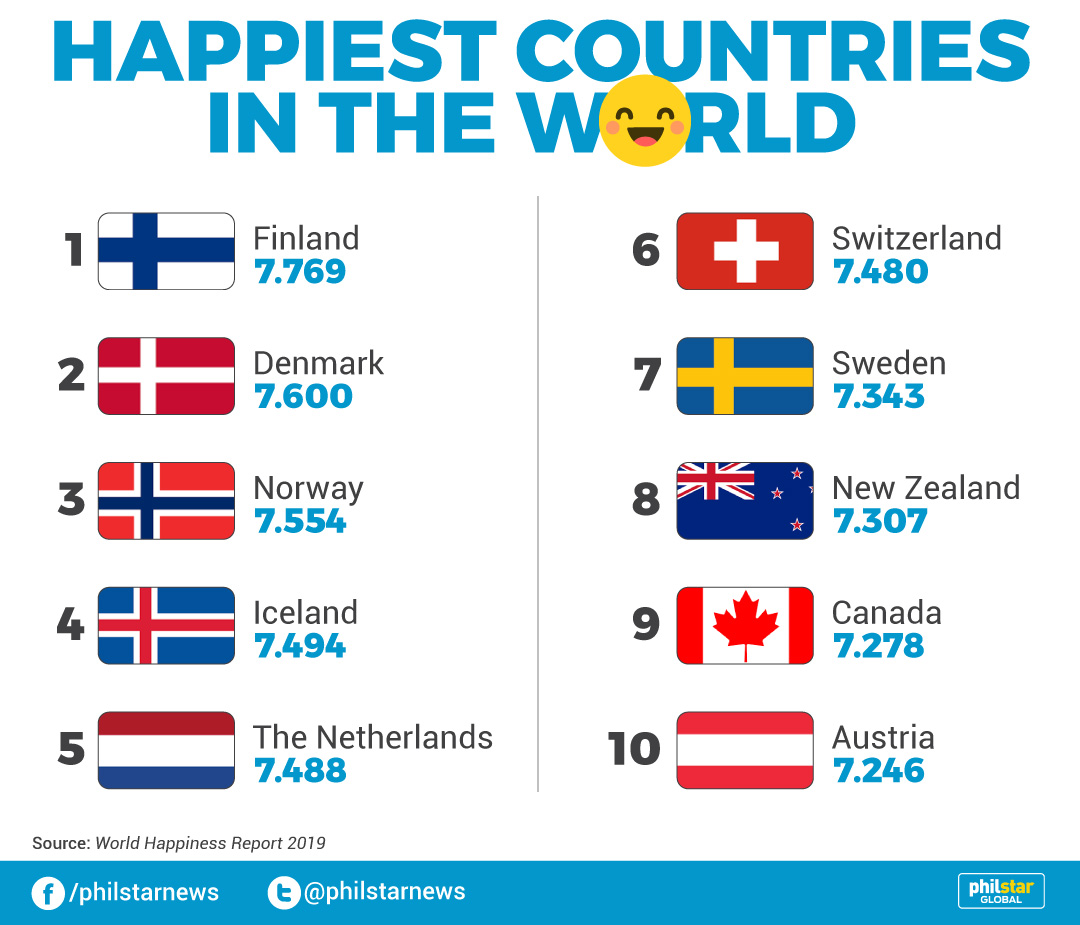
\includegraphics[height=.65\textheight]{../figures/happiest_countries.jpg}}
    \ip The answer is often a \rose{Scandinavian}, \blue{high-income country}. 
    % \ip What do we mean by ``happy''? \pause Subjective well-being.
    \ip Is money really buying happiness?
    \ee
\end{frame}

\begin{frame}{Literature}
    \bbsp
    \ip \centering \only<1>{World Values Survey, $R^2=.49$ (Inglehart \& Klingemann, 2000) \\
    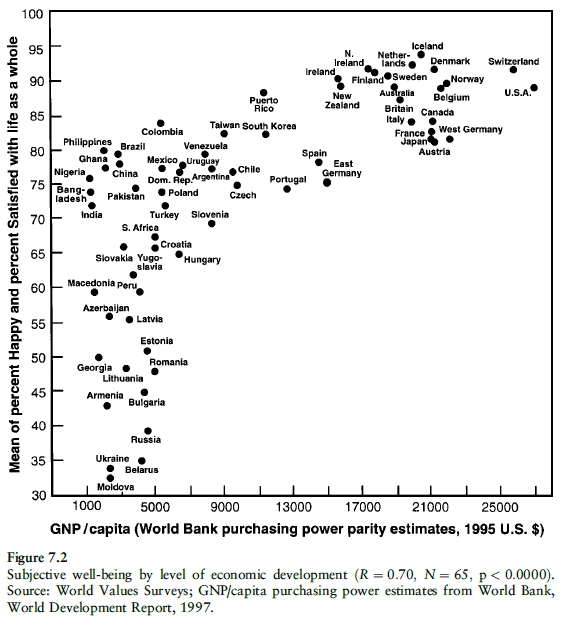
\includegraphics[height=.8\textheight]{../figures/Inglehart_Klingemann}}
    \only<2>{World Happiness Report (Gallup, 2023) \\
    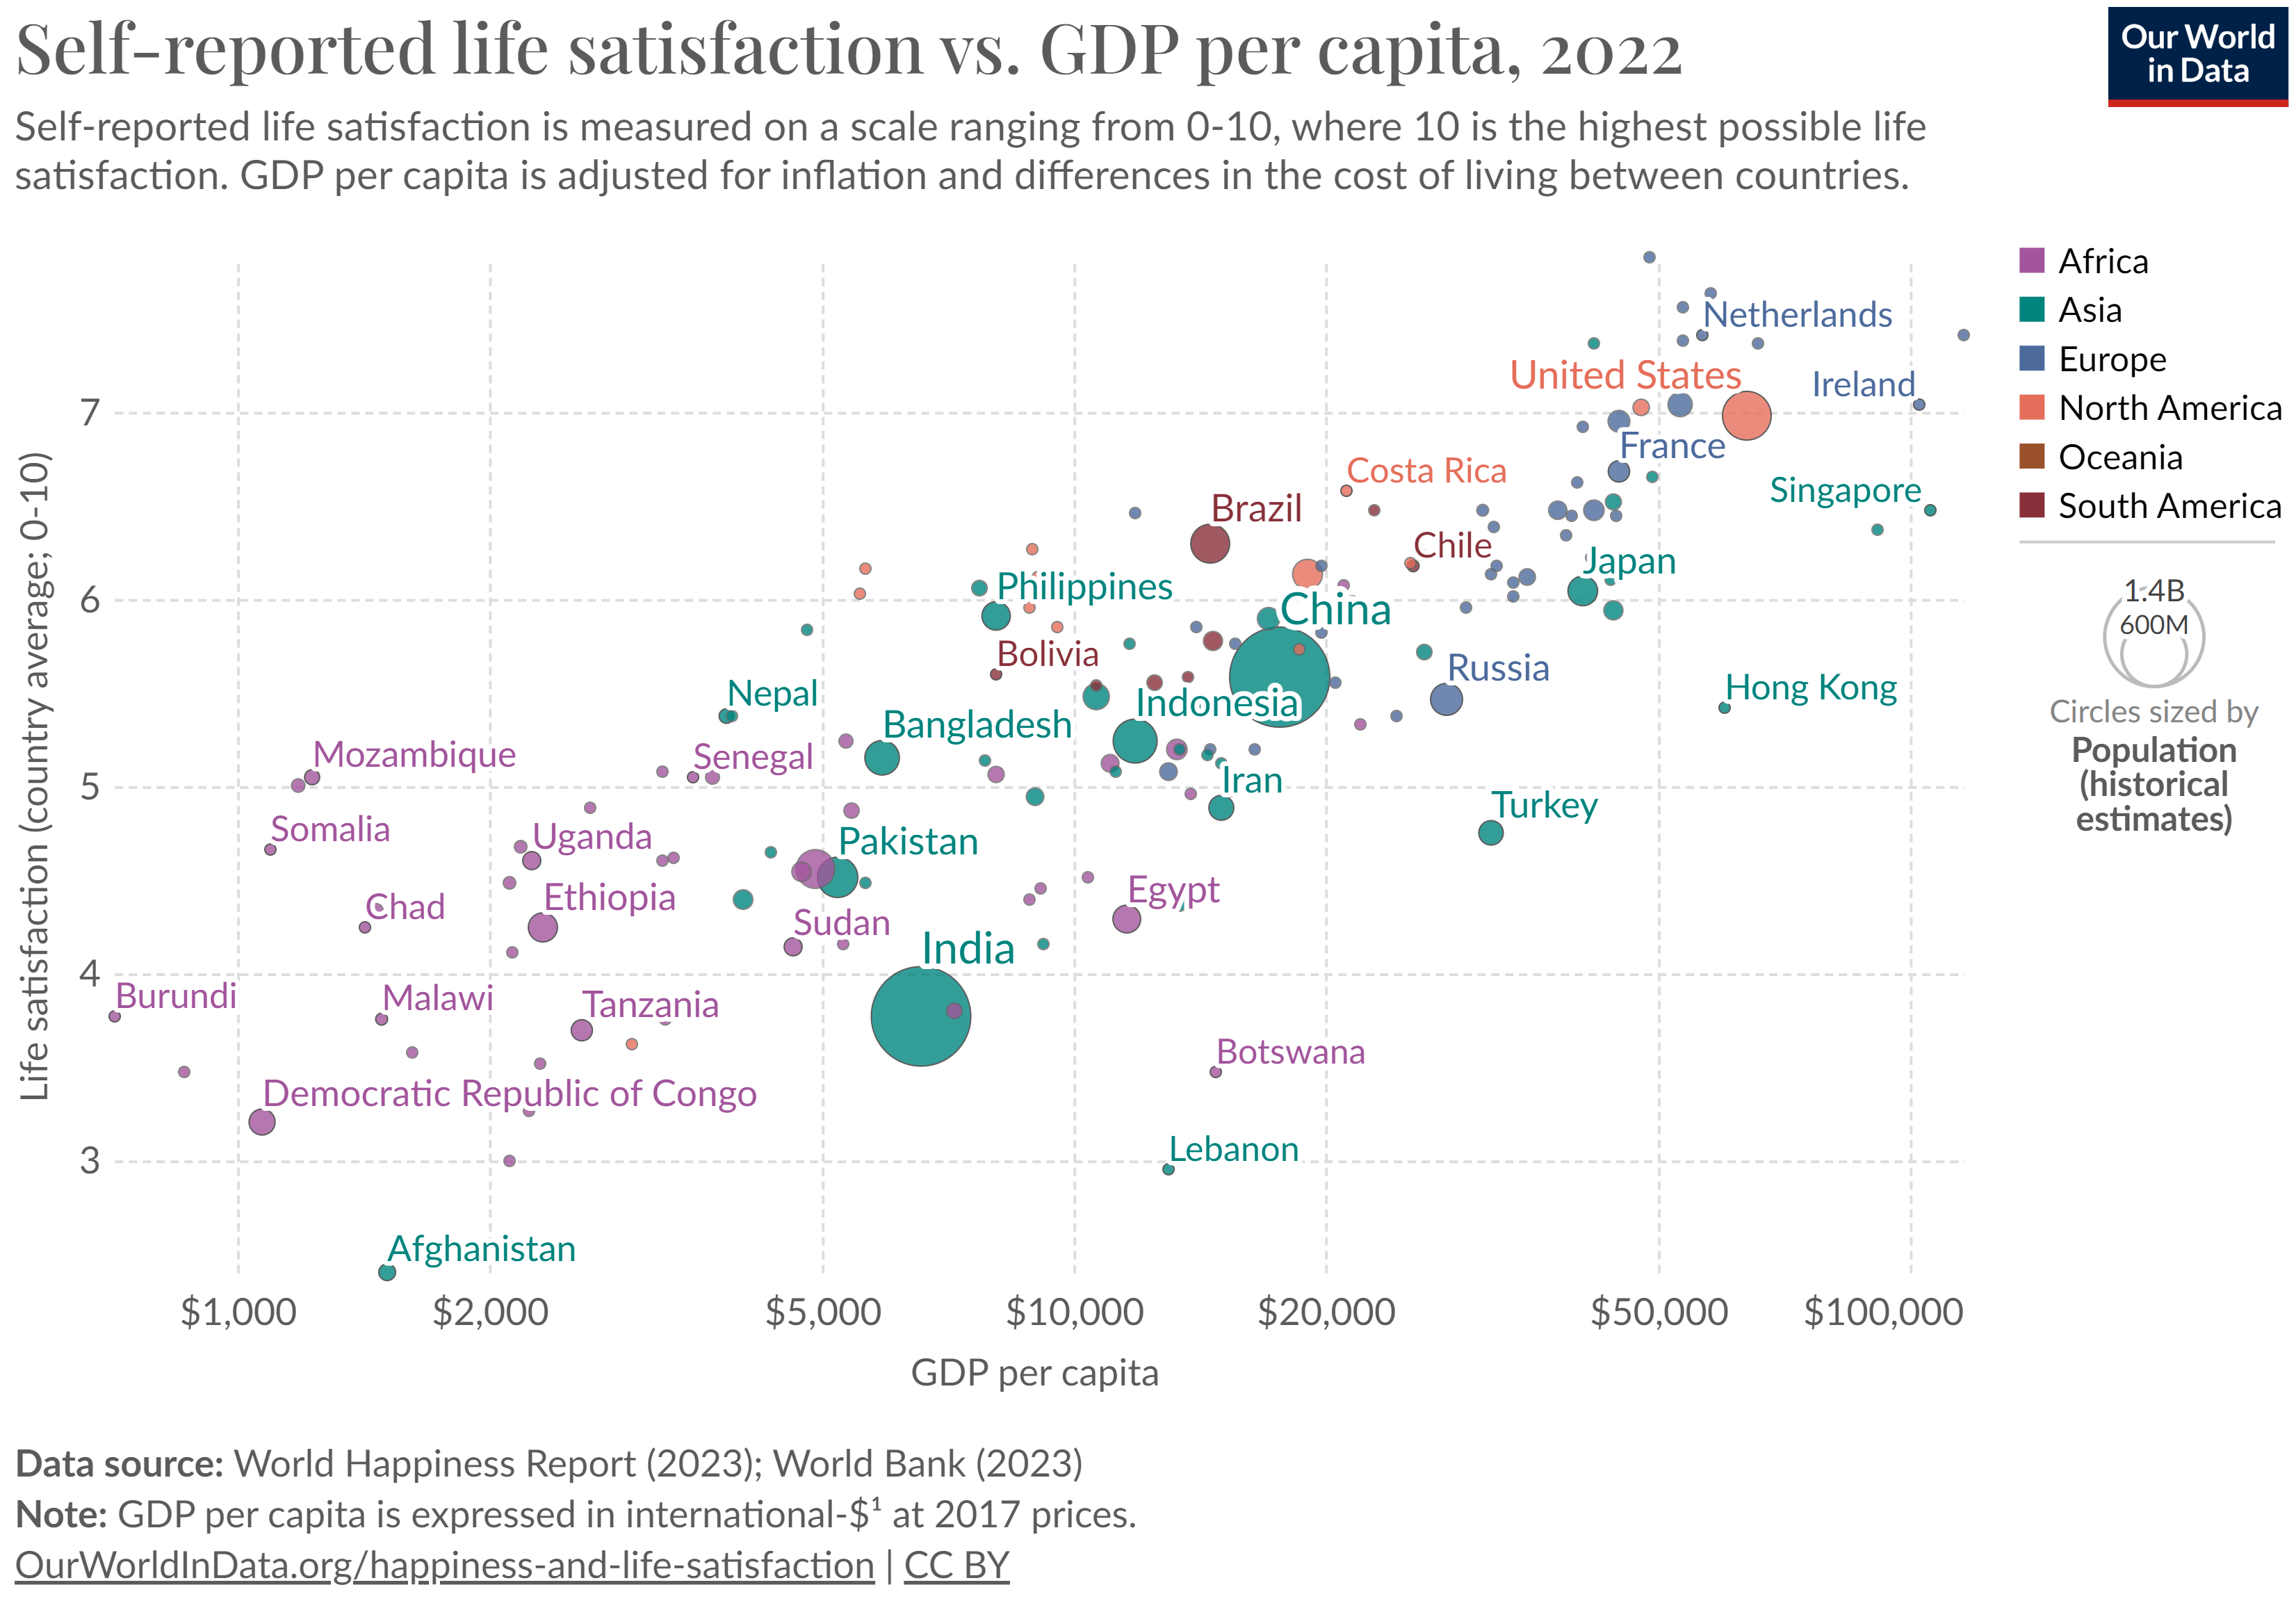
\includegraphics[height=.75\textheight]{../figures/owid_satisfaction_gdp}}
    \ip The literature finds an \blue{increasing relationship between GDP pc and well-being}.
    \ip Deaton (2008) finds a log-linear relation between average satisfaction and GDP pc PPP using Gallup data ($R^2=.71$).
    \ip Latin America (Eastern Europe) is (un)happier than predicted (Inglehart et al., 2008).
    \ip 
    Gallup question shows stronger correlation than World Values Survey's (Deaton, 2008).
    \ip National income is more correlated to satisfaction than to happiness (Deaton, 08).% Inglehart et al., 2008
    \ip Blanchflower \& Bryson (2023) document different countries' rankings in terms of positive and negative affects.
    % Original graph is Inglehart & Klingemann (00)
    % https://ourworldindata.org/grapher/gdp-vs-happiness World Happiness Report
    % https://www.digitalinformationworld.com/2023/04/data-shows-correlation-between-gdp-per.html same source
    % https://econreview.berkeley.edu/beyond-gdp-economics-and-happiness/ same discourse as mine, The Economist chart
    % World Happiness Index and GDP per capita have correlation of .84, "same thing" for Salvatores Babones https://twitter.com/ProfBabones/status/1638924519510519809
    % various references https://www.maxroser.com/roser/notebook/happiness/
    % Great article: https://ourworldindata.org/happiness-and-life-satisfaction (already showing specificity of Latin America)
    \ip \rose{We} study new indicators and \\ \rose{challenge the view that national income is the best predictor of well-being}.
    % CITE: 
    % Deaton (08): log-linear relation satisfaction - GDP pc PPP using Gallup (r = .84)
    % WHR (23)
    % Di Tella et al. (07): people adapt to new income after 4 years 
    % Inglehart et al. (08): drivers of national WB. Income linked to satisfaction more than happiness, and many other things
    % Blanchflower & Bryson (23): rankings of diff well-being indicators 
    % CITE only in the paper (or perhaps not): Oishi et al. (21); Deaton (08); Killingsworth et al. (23); Clark..; 
    % Sandvik et al., 93: SWB is a reliable indicator (corresponds to objective measures or judgments by others); Lucas & Diener (99,09): SWB linked to personality (in particular extraversion and neuroticism, and all are stable)
    \ee
\end{frame}

\begin{frame}{Primer of the results}
    \bbsp
    \ip \rose{Income is only weakly correlated with national well-being}.
    \ip The relationship heavily depends on the well-being indicator chosen. \pause \\ For some indicators, the happiest country is in Africa or Latin America.\pause
    \ip Another simple variable, the country's (macro) \rose{region}, \rose{is a better predictor} of national well-being.
    \ee
\end{frame}

\section{Design}

\begin{frame}{Data}
    \bbvsp
    \ip \blue{World Values Survey} (\blue{WVS}): representative surveys on 440,000 respondents over 108 countries.
    \ip 304 country $\times$ year observations among 7 waves from 1981 to 2022.
    \ip Two subjective well-being questions:
    \bbvsp 
    \ip \rose{Happiness}: ``Taking all things together, \blue{would you say you are}:'' \\ ~\textit{\blue{Very happy}}; \textit{\blue{Quite happy}}; \textit{\blue{Not very happy}}; \textit{\blue{Not at all happy}}; PNR % Q46
    \ip \rose{Satisfaction}: ``All things considered, \blue{how satisfied are you with your life as a whole these days?}'' \textit{\blue{1}-Completely dissatisfied} -- \textit{\blue{10}-Completeley satisfied}; PNR % Please use this card to help with your answer.
    \ee
    \ee
    \centering 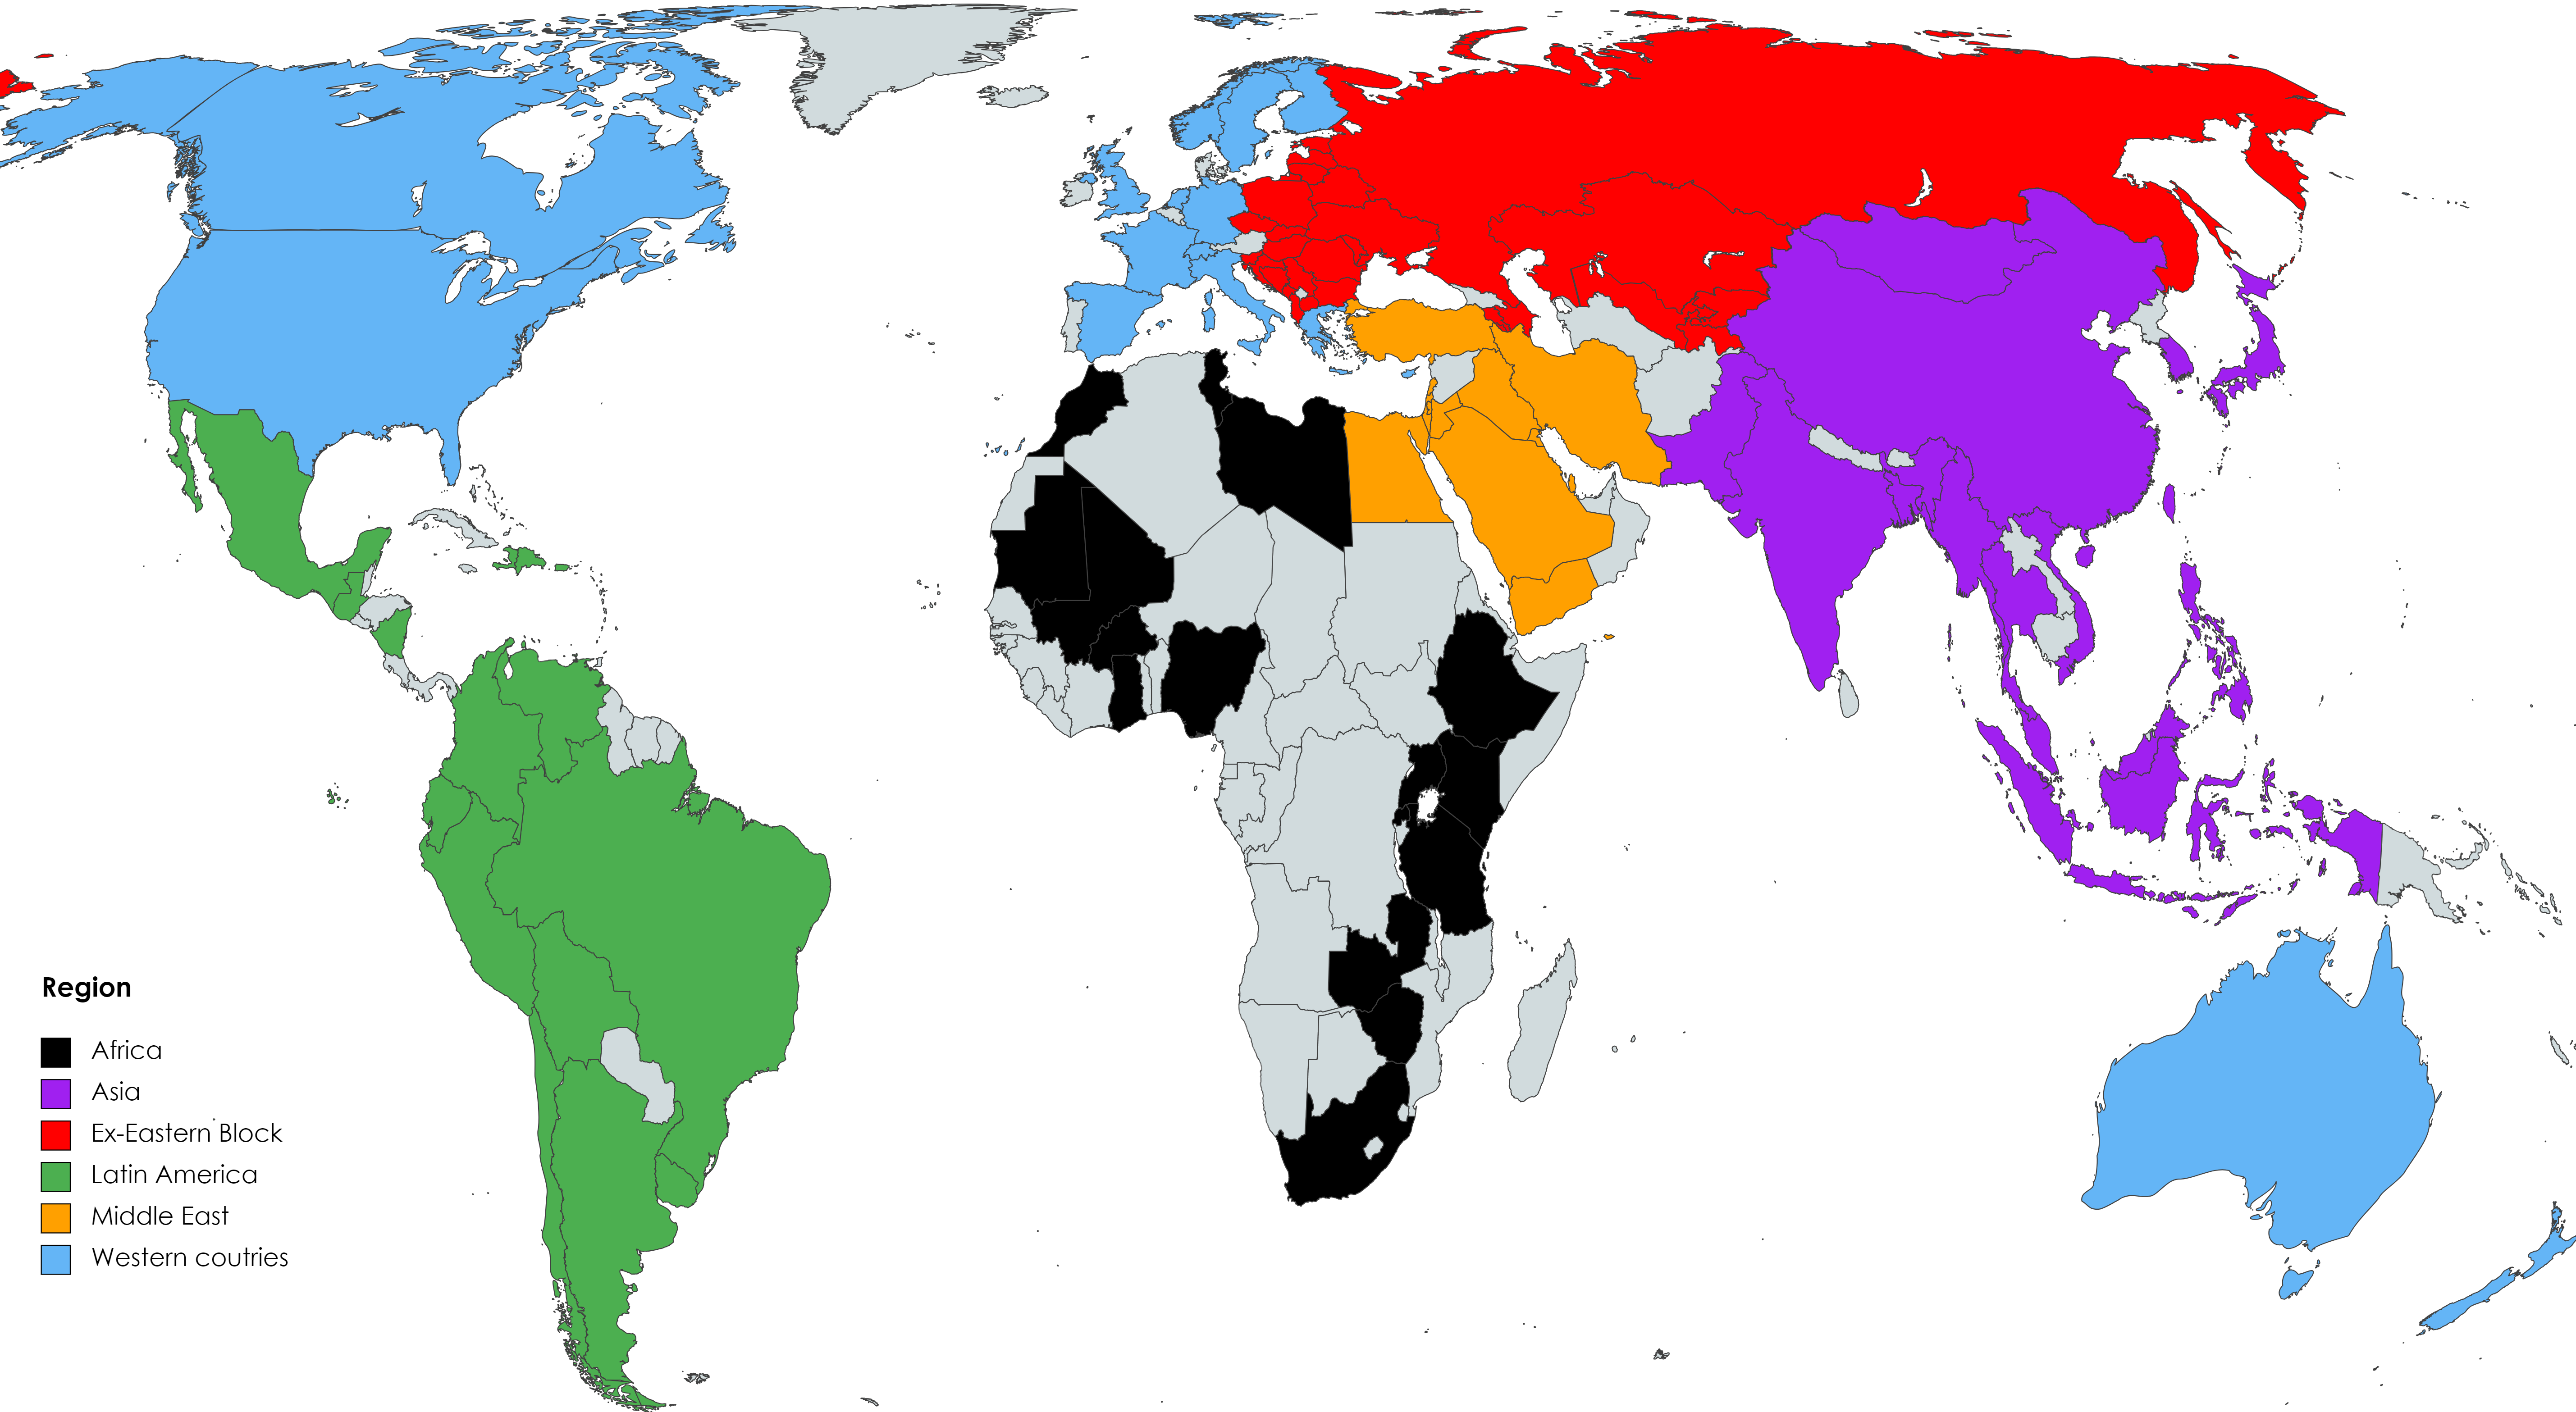
\includegraphics[height=.5\textheight]{../figures/WVS_countries_regions}
\end{frame}

\begin{frame}{What is national well-being?}
    With the two well-being questions, \blue{we can define various} national \blue{indicators} (all weighted using survey weights, all excluding PNR).
    \bbvsp
    \ip \textbf{\blue{Happy}}: share answering \textit{Quite} or \textit{Very happy}
    \ip \textbf{\blue{Very Happy}}: share answering \textit{Very happy}
    \ip \textbf{\blue{Very Unhappy}}: share answering \textit{Very unhappy}
    \ip \textbf{\blue{V. Happy -- V. Unhappy}}: difference \textbf{Very Happy} minus \textbf{Very Unhappy}
    \ip \textbf{\blue{Happiness (mean)}}: mean happiness recoded into $-$3; $-$1; +1; +3
    \ip \textbf{\blue{Satisfaction (mean)}}: mean satisfaction
    \ip \textbf{\blue{Satisfied}}: share answering 6 to 10 at satisfaction
    \ip \textbf{\blue{Happy + Satisfied}}: average of \textbf{Happy} and \textbf{Satisfied}\\ ~\quad This is the variable used by Inglehart \& Klingemann (2000) % https://www.staff.ncl.ac.uk/david.harvey/MKT3008/IntDev/happiness&GDP.gif SWB index by Inglehart & Klingemann (00)
    \ip Bond \& Lang (19) show that no single indicator can reliably identify two group's relative well-being, justifying reliance on several indicators.
    \ee 
\end{frame}
% TODO: plot happy against satisfied

\begin{frame}{How we measure income}    
    \bbsp % As usual in this literature, (e.g. WHR23, Inglehart 08)
    \ip Our benchmark \textit{income} indicator is the \blue{\textbf{log} GDP per capita (pc) in \textbf{PPP}} (constant 2017 \$, World Bank) \pause \\ We also use discrete indicators: \pause \bbsp
    \ip \textbf{\blue{Income sextile}}: quantile of income (6 quantiles)
    \ip \textbf{\blue{Income cluster}} (\textit{k} = \textbf{5}, \textbf{6} or \textbf{7}): income cluster, with the \textit{k} clusters found by the \textit{k}-means algorithm
    \ee
    \ip For robustness, we also run our analyses using the log \textit{nominal} GDP pc (constant 2015 \$, World Bank) and corresponding income group and clusters.
    \ip We manually impute missing income data using IMF data.
    \bbsp \ip For robustness, we also run our analyses without this imputation (excluding countries with missing GDP data).
    \ee
    \ee 
\end{frame}

\section{National well-being and income}

\begin{frame}{Graphical evidence}
\begin{figure}
    \only<+>{\caption{\textbf{Happy} vs. log GDP p.c. (PPP) --- All waves of WVS.} \vspace{-.3cm}
    \centering 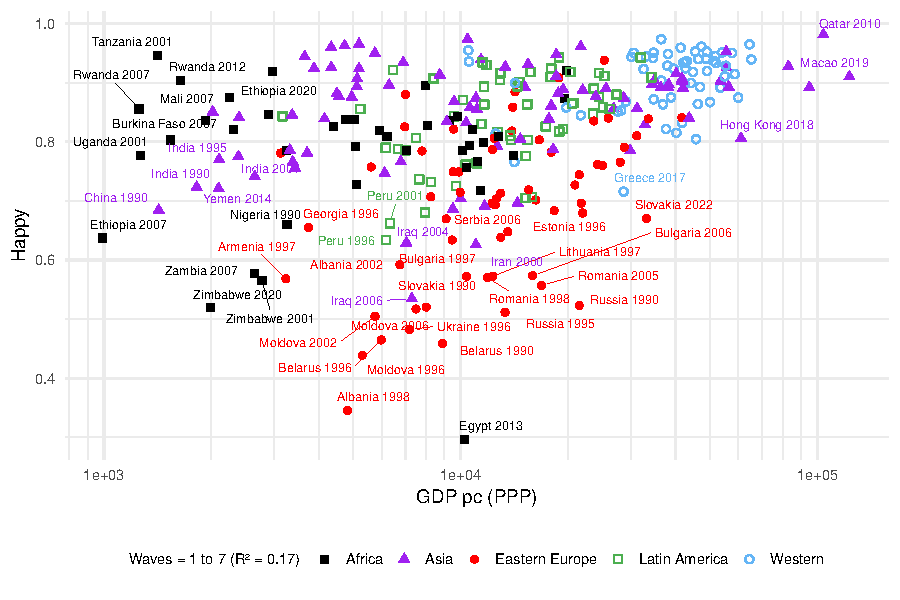
\includegraphics[height=.9\textheight]{../figures/happy_vs_GDPppp.pdf}}
    \only<+>{\caption{\textbf{Very Happy} vs. log GDP p.c. (PPP) --- All waves of WVS.}  \vspace{-.3cm}
    \centering 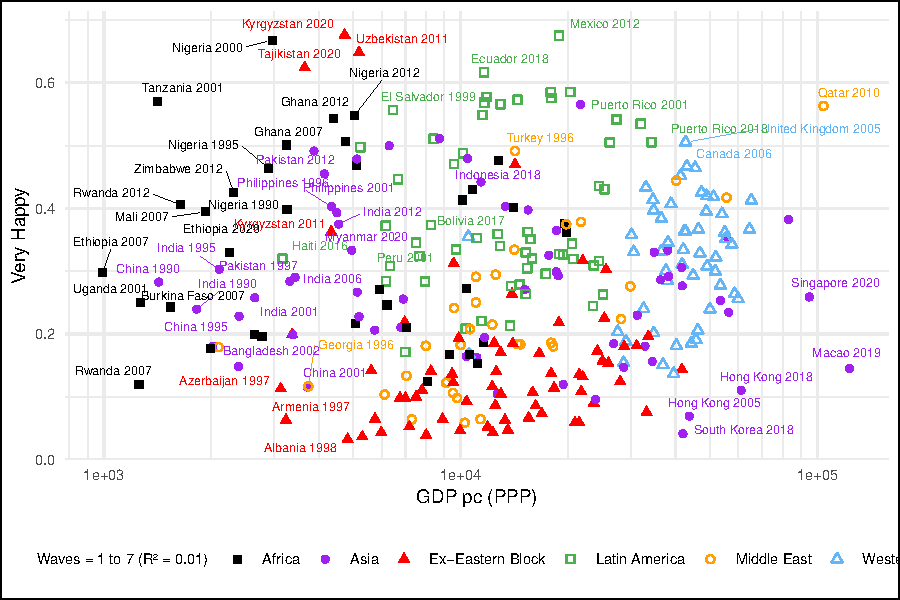
\includegraphics[height=.9\textheight]{../figures/very_happy_vs_GDPppp.pdf}}
    \only<+>{\caption{\textbf{Very Unhappy} vs. log GDP p.c. (PPP) --- All waves of WVS.}  \vspace{-.3cm}
    \centering 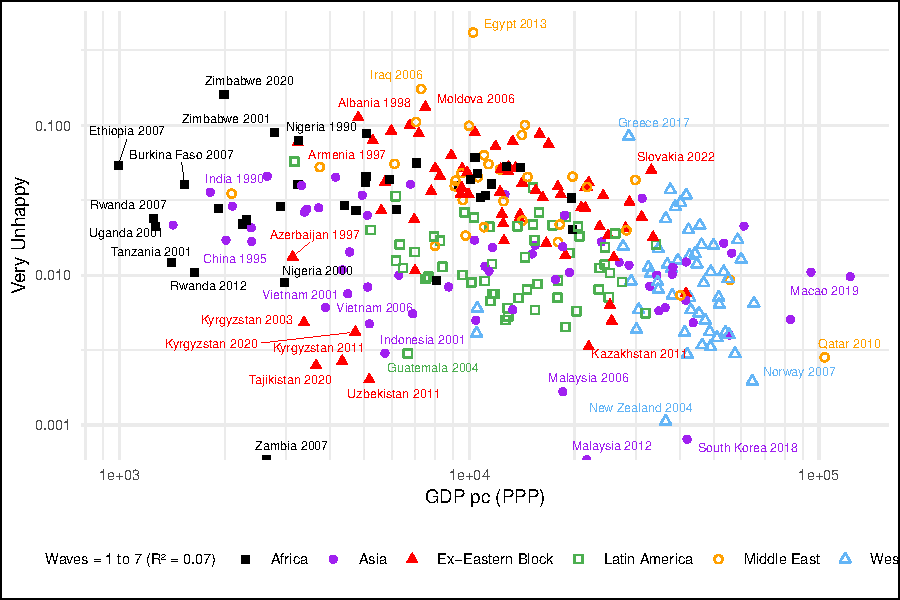
\includegraphics[height=.9\textheight]{../figures/very_unhappy_vs_GDPppp.pdf}}
    \only<+>{\caption{\textbf{V. Happy -- V. Unhappy} vs. log GDP p.c. (PPP) --- All waves of WVS.} \vspace{-.3cm}
    \centering 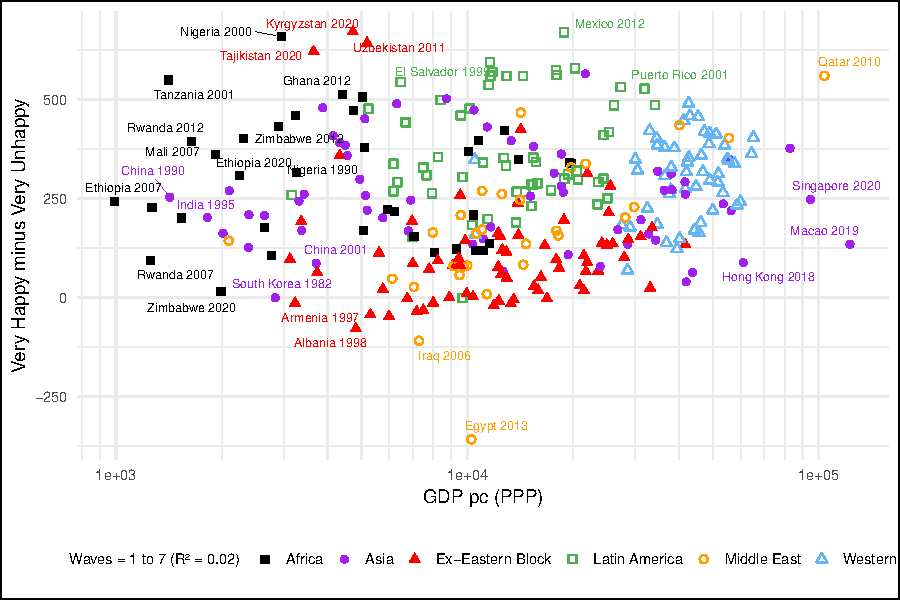
\includegraphics[height=.9\textheight]{../figures/very_happy_minus_very_unhappy_vs_GDPppp.pdf}}
    \only<+>{\caption{\textbf{Happiness (mean)} vs. log GDP p.c. (PPP) --- All waves of WVS.}  \vspace{-.3cm}
    \centering 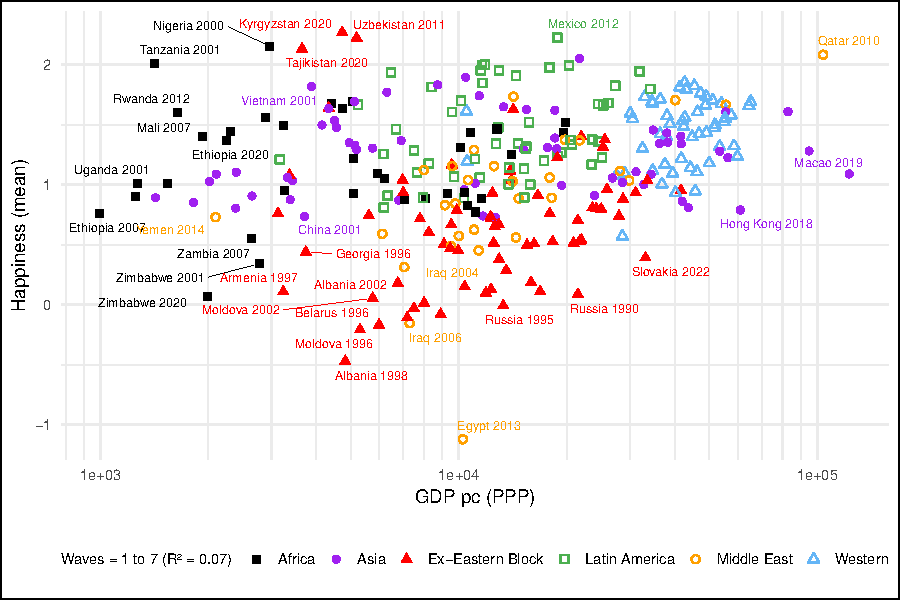
\includegraphics[height=.9\textheight]{../figures/happiness_mean_vs_GDPppp.pdf}}
    \only<+>{\caption{\textbf{Satisfaction (mean)} vs. log GDP p.c. (PPP) --- All waves of WVS.}  \vspace{-.3cm}
    \centering 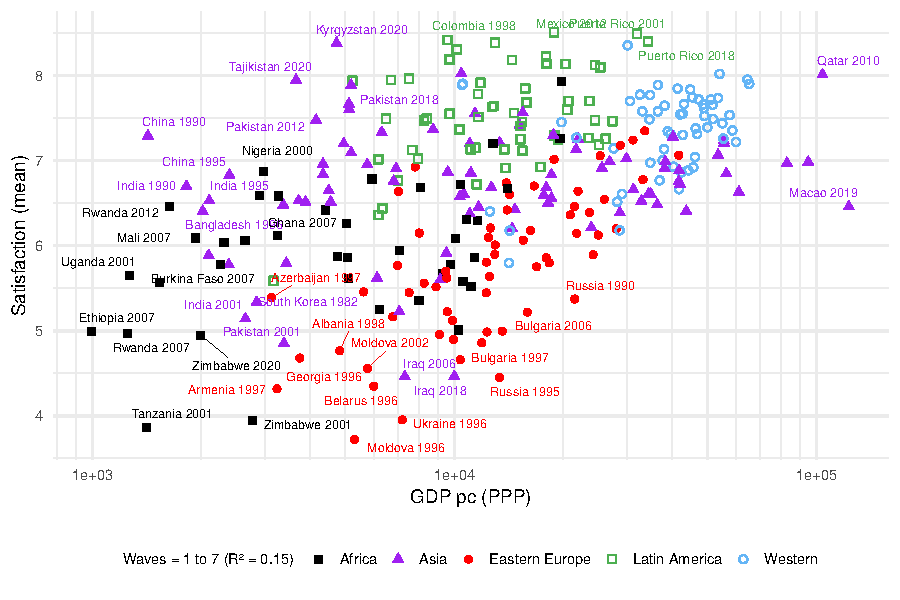
\includegraphics[height=.9\textheight]{../figures/satisfied_mean_vs_GDPppp.pdf}}
    \only<+>{\caption{\textbf{Satisfied} vs. log GDP p.c. (PPP) --- All waves of WVS.} 
    \centering \vspace{-.3cm} 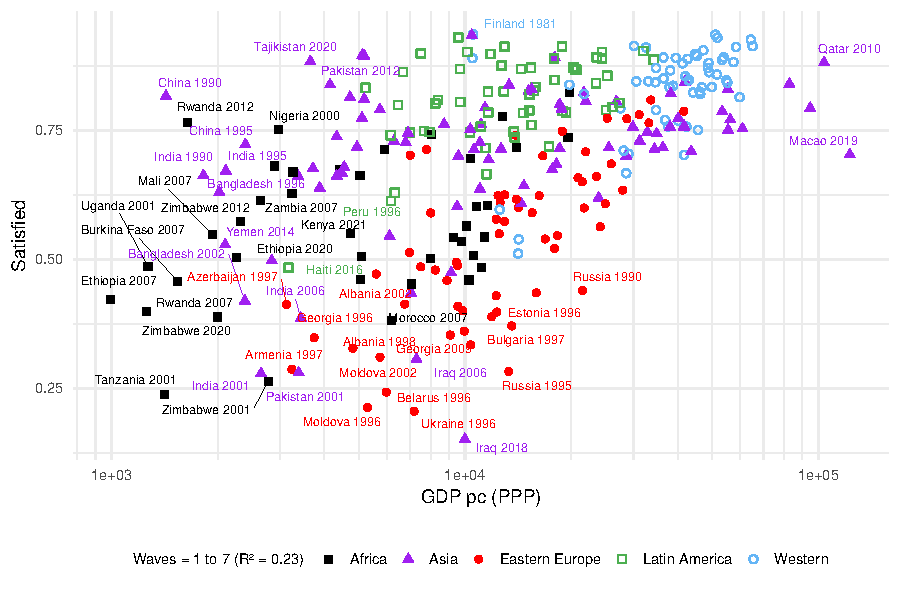
\includegraphics[height=.9\textheight]{../figures/satisfied_vs_GDPppp.pdf}}
    \only<+>{\caption{\textbf{Happy + Satisfied} vs. log GDP p.c. (PPP) --- All waves of WVS.}  \vspace{-.3cm}
    \centering 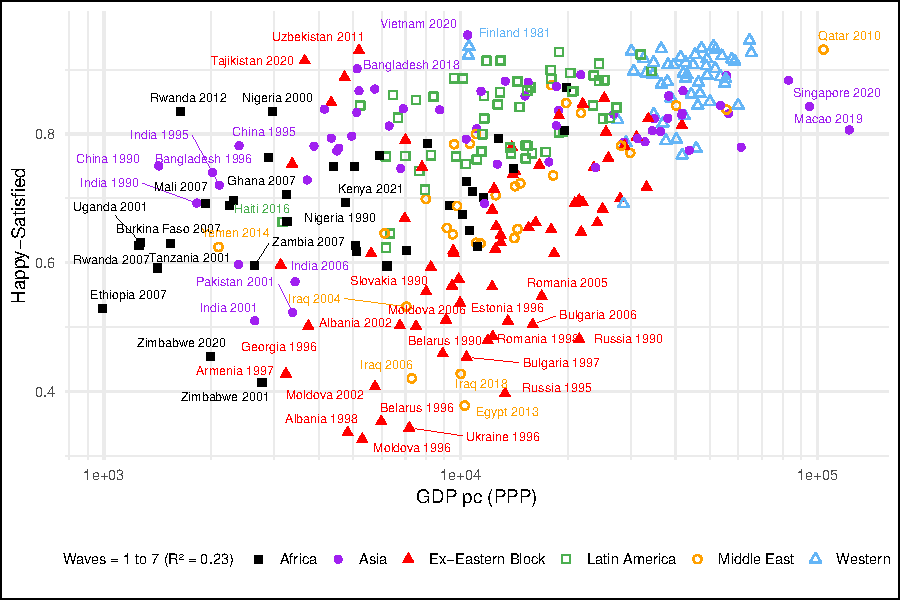
\includegraphics[height=.9\textheight]{../figures/happiness_Layard_vs_GDPppp.pdf}}
    \only<+>{\caption{\textbf{Happy} vs. log GDP p.c. (nominal) --- Wave 7 (2017-22) of WVS, weighted by population.}  \vspace{-.3cm}
    \centering 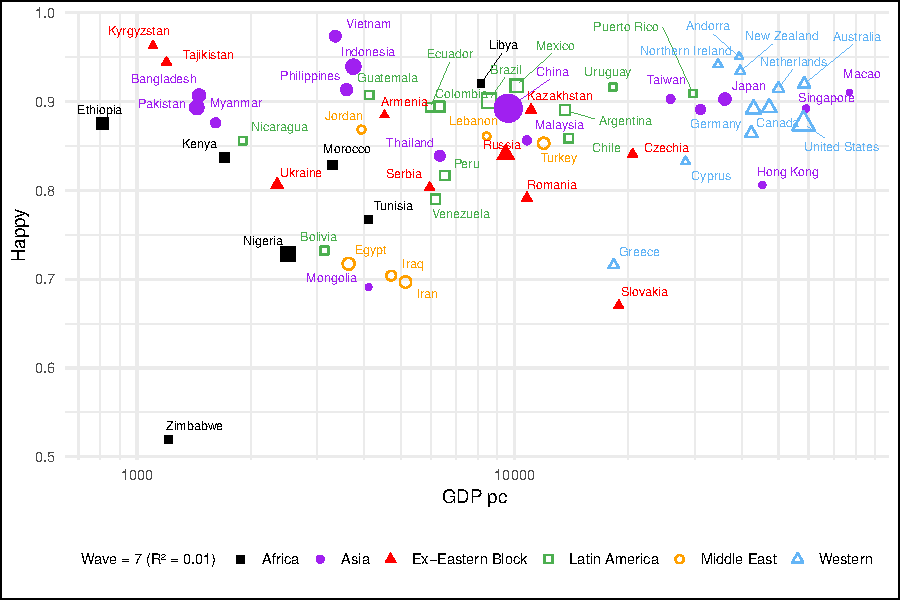
\includegraphics[height=.9\textheight]{../figures/happy_vs_GDP_wave7_weighted.pdf}}
\end{figure}
\end{frame}

\begin{frame}{Variance explained by GDP p.c.\label{gdp} \hyperlink{gdp_add}{\beamergotobutton{More results}}}
    \only<2>{
\begin{tabular}[t]{lccccccccc}
\toprule Happiness variable & \multicolumn{2}{c}{log GDP p.c.} & \multicolumn{5}{c}{Income cluster} & & \\
  & \makecell{\,\\PPP} & \makecell{\,\\nominal} & \makecell{sextile\\PPP} & \makecell{k = 5\\PPP} & \makecell{k = 6\\PPP} & \makecell{k = 7\\PPP} & \makecell{k = 7\\nominal} & Mean & Max\\
\midrule
Satisfied & 0.41 & 0.46 & 0.36 & 0.41 & 0.41 & 0.45 & 0.47 & 0.42 & 0.47\\
NA & 0.24 & 0.32 & 0.24 & 0.27 & 0.27 & 0.28 & 0.32 & 0.28 & 0.32\\
NA & 0.06 & 0.11 & 0.1 & 0.08 & 0.08 & 0.09 & 0.13 & 0.09 & 0.13\\
NA & 0.01 & 0 & 0.06 & 0.03 & 0.03 & 0.04 & 0.02 & 0.03 & 0.06\\
NA & 0.35 & 0.36 & 0.26 & 0.34 & 0.33 & 0.39 & 0.41 & 0.35 & 0.41\\
NA & 0.33 & 0.32 & 0.26 & 0.34 & 0.31 & 0.38 & 0.38 & 0.33 & 0.38\\
Satisfaction (mean) & 0.01 & 0.02 & 0.05 & 0.05 & 0.06 & 0.06 & 0.08 & 0.05 & 0.08\\ \midrule 
Mean & 0.2 & 0.23 & 0.19 & 0.22 & 0.21 & 0.24 & 0.26 & 0.22 & 0.26\\
Max & 0.41 & 0.46 & 0.36 & 0.41 & 0.41 & 0.45 & 0.47 & 0.42 & 0.47\\ \midrule 
Number of obs. & 142 & 142 & 142 & 142 & 142 & 142 & 142 &  & \\
\bottomrule
\end{tabular}}
    \only<1,3->{
    \bbsp
    \ip For different \textit{well-being} and \textit{income} indicators, we compute the $R^2$ of the regression: $$well\text{-}being_i = \alpha + \beta\, income_i + u_i$$ \pause
    \ip \rose{\textbf{Nominal income clustered into 7 groups}} is the income indicator that \rose{explains best well-being}.
    \ip On average over well-being indicators, \blue{this indicator explains 13\% of the variance}.
    \ip \blue{\textbf{Satisfied} is the well-being indicator that is best explained }by income (19\% to 24\%).
    \ip \textbf{Happy + Satisfied} ---chosen by Ingelhart et al. (2008)--- comes close (17\% to 23\%).
    \ip \blue{\textbf{Happiness (mean)} is poorly explained} by income (8\% at best).
    \ee
    }
\end{frame}

\begin{frame}{What are the happiest countries?}
    \bbvsp
    \ip \blue{What is the happiest country?}
    \ip Looking at all waves combined, \rose{Kyrgyzstan}--2020 is the happiest country--year according to 3 indicators\\Finland, Malaysia, Mexico, Qatar, Vietnam according to other indicators.
    \ip Counting the occurrences of countries for each wave--indicator (including all waves combined), \blue{Switzerland} is the happiest (10 occurrences) followed by \blue{Mexico} (9) and \blue{Kyrgyzstan} (6).
    \ip The happiest countries are Western (24), in Latin America (19), Asia (16) or Africa (6).
    \ip Blanchflower \& Bryson (2023) show that on respective positive/negative affects, the happiest state is: Bhutan (well-rested), Denmark (satisfaction), Finland (anger), Hawaï (enjoy), Paraguay (smile), Taiwan (sadness), Uzbekistan (worry), Vietnam (pain). % Paraguay 1st on overall positive, Taiwan on negative, Hawaï on total
    \ee
\end{frame}

% Results: TODO Some indicators are not significantly related with GDP per capita, while some others (like the share of very happy people) are even decreasing with GDP per capita
% Results: TODO table of happiest countries

\section{Region vs. GDP per capita\\as predictor of well-being}

\begin{frame}{Region grouping}
    \begin{figure}
        \caption{WVS countries grouped into the five UN regional groups.}  
        \centering 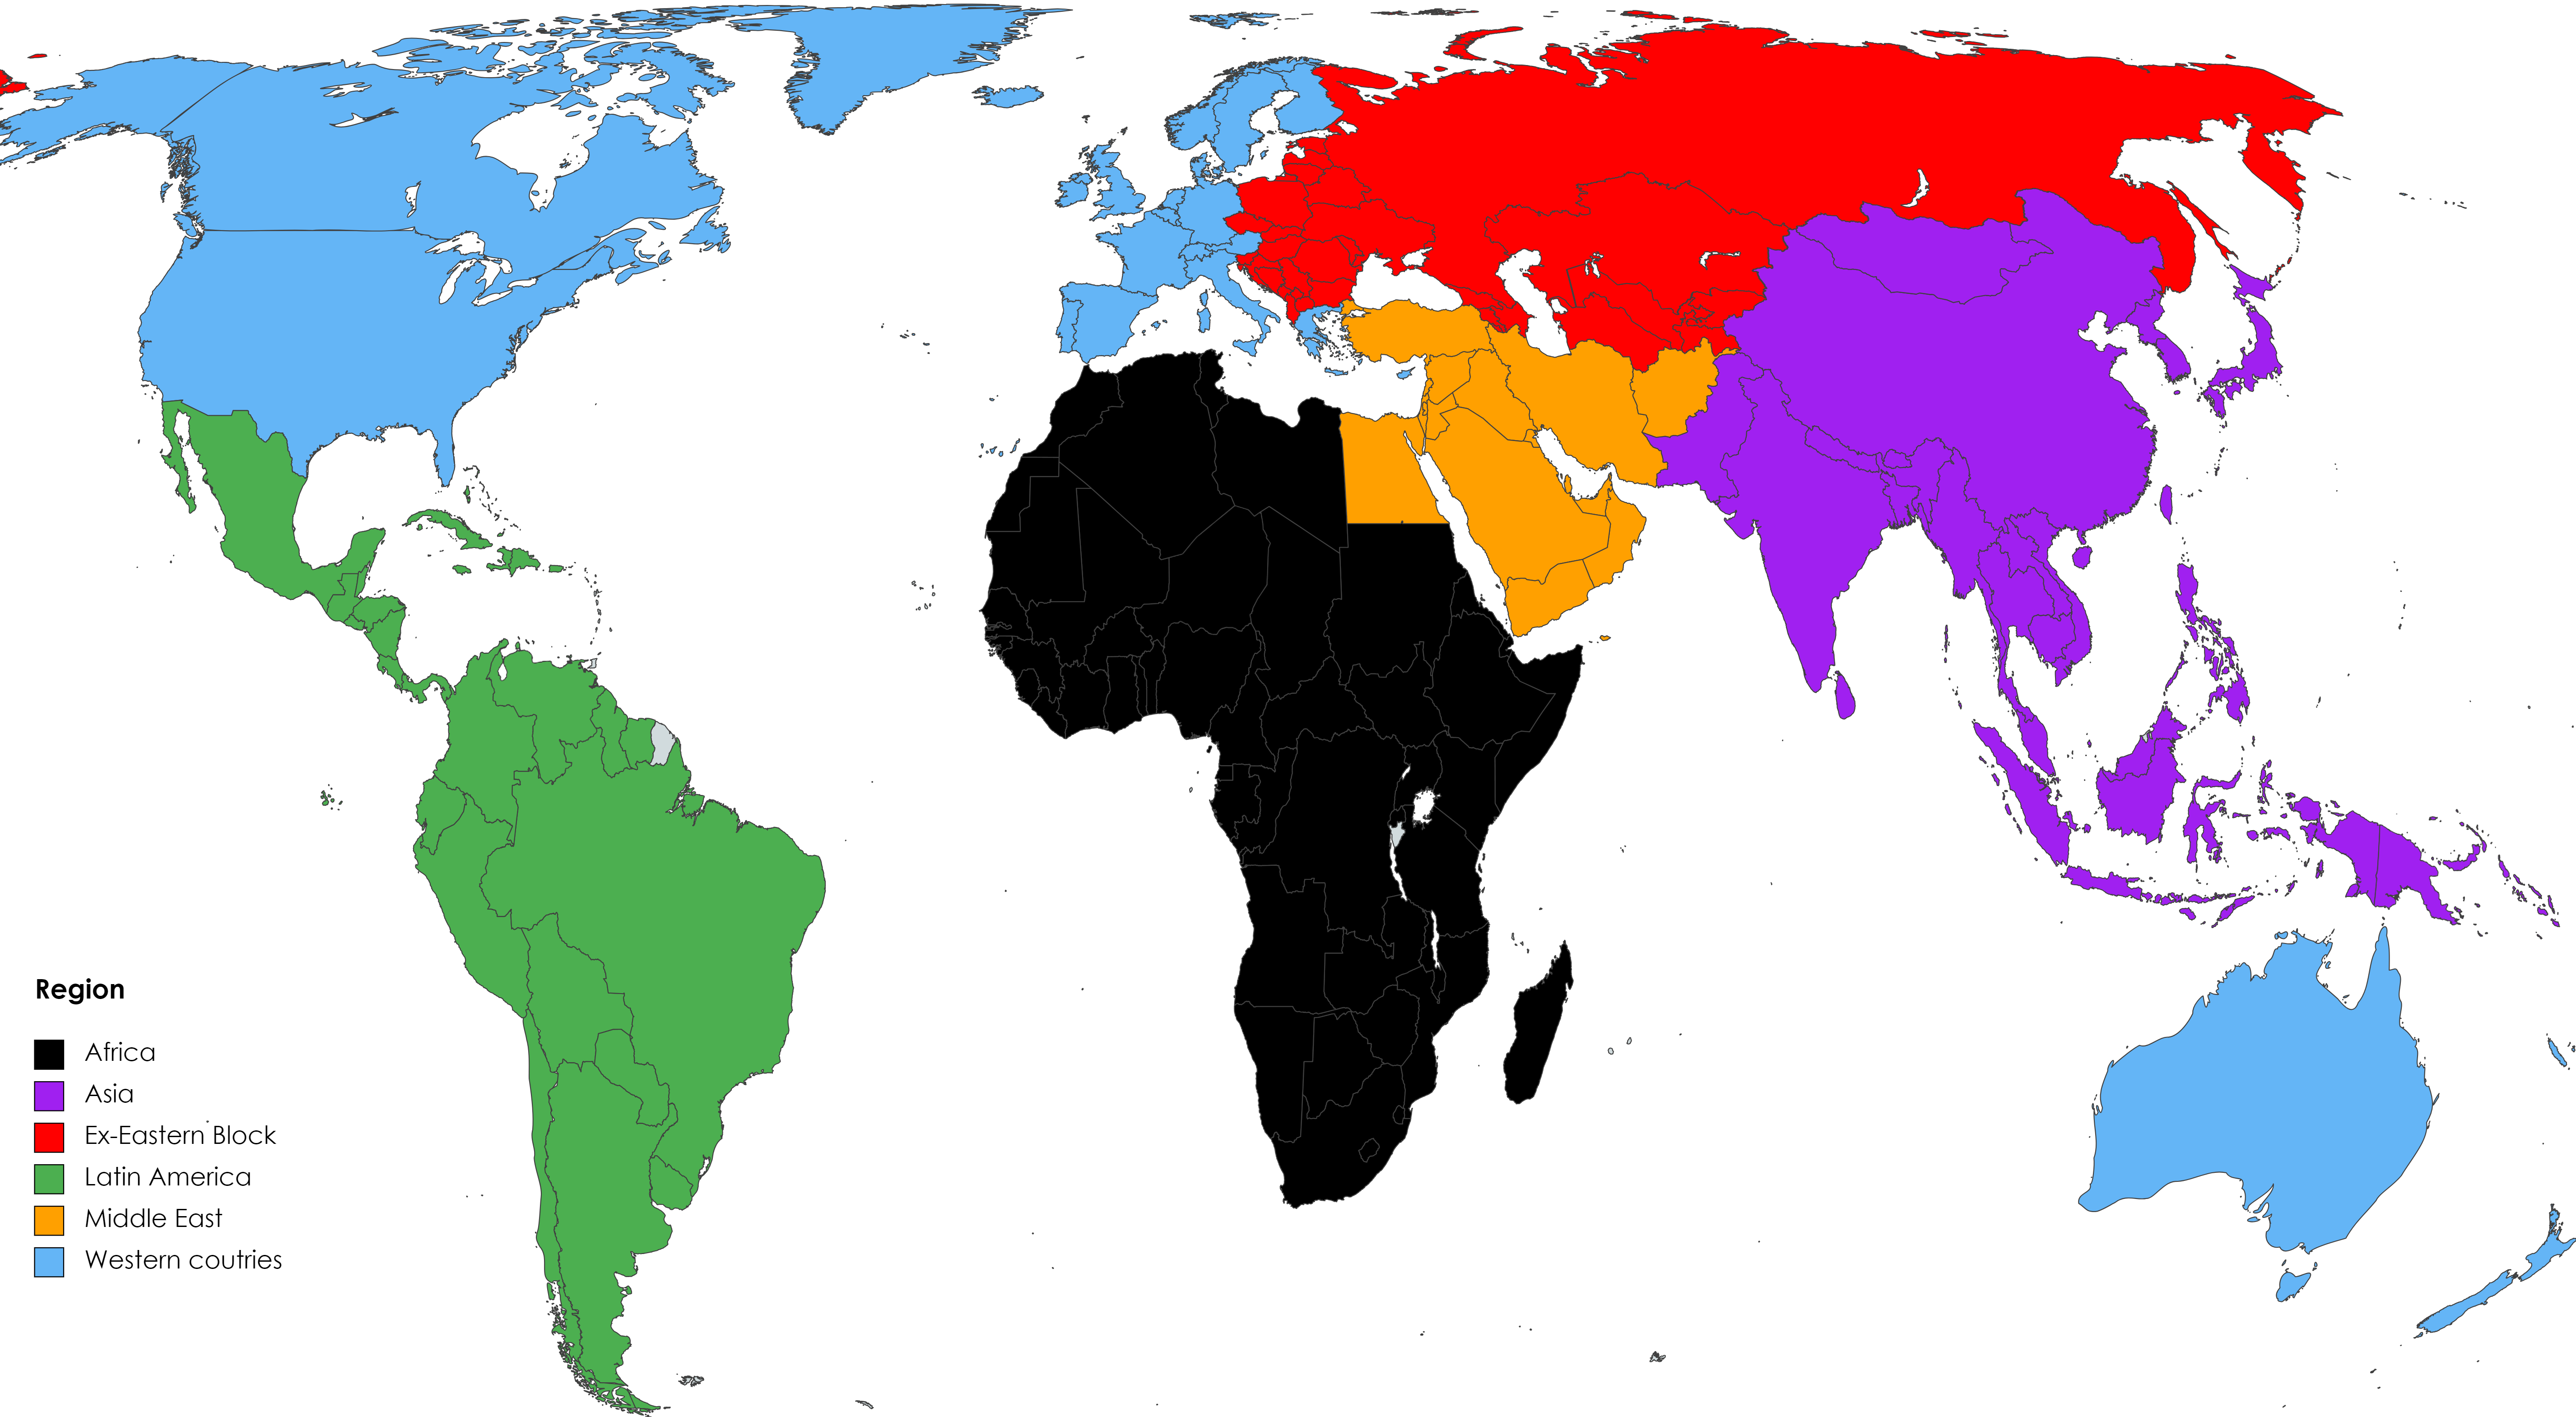
\includegraphics[height=.8\textheight]{../figures/region_groupings} % region_groupings
    \end{figure}
\end{frame}

\begin{frame}{Comparing the share of variance explained by income vs. region}
    % \only<6>{
\begin{tabular}[t]{lccccccccc}
\toprule Happiness variable & \multicolumn{2}{c}{log GDP p.c.} & \multicolumn{5}{c}{Income cluster} & & \\
  & \makecell{\,\\PPP} & \makecell{\,\\nominal} & \makecell{sextile\\PPP} & \makecell{k = 5\\PPP} & \makecell{k = 6\\PPP} & \makecell{k = 7\\PPP} & \makecell{k = 7\\nominal} & Mean & Max\\
\midrule
Very Happy & 0 & 0.01 & 0.13 & 0.03 & 0.04 & 0.07 & 0.12 & 0.06 & 0.13\\
Happy & 0.27 & 0.33 & 0.36 & 0.34 & 0.33 & 0.34 & 0.39 & 0.34 & 0.39\\
Very Unhappy & 0.19 & 0.25 & 0.27 & 0.27 & 0.27 & 0.26 & 0.38 & 0.27 & 0.38\\
Satisfied & 0.36 & 0.42 & 0.35 & 0.37 & 0.39 & 0.38 & 0.44 & 0.39 & 0.44\\
Satisfaction (mean) & 0.27 & 0.32 & 0.26 & 0.27 & 0.29 & 0.28 & 0.34 & 0.29 & 0.34\\
Happiness (mean) & 0.1 & 0.14 & 0.21 & 0.16 & 0.15 & 0.17 & 0.22 & 0.16 & 0.22\\
Happy + Satisfied & 0.33 & 0.4 & 0.36 & 0.36 & 0.37 & 0.37 & 0.43 & 0.38 & 0.43\\
V. Happy -- V. Unhappy & 0.02 & 0.03 & 0.14 & 0.06 & 0.06 & 0.09 & 0.14 & 0.08 & 0.14\\ \midrule 
Mean & 0.19 & 0.24 & 0.26 & 0.23 & 0.24 & 0.24 & 0.31 & 0.24 & 0.31\\
Max & 0.36 & 0.42 & 0.36 & 0.37 & 0.39 & 0.38 & 0.44 & 0.39 & 0.44\\ \midrule 
Number of obs. & 304 & 304 & 304 & 304 & 304 & 304 & 304 &  & \\
\bottomrule
\end{tabular}}
    % \only<1-5,7->{
    \bbvsp
    \ip For different \textit{well-being} and \textit{income} indicators, we run regressions and compute corresponding $R^2$: 
    % \ee    
    % \makebox[.7\textwidth][c]{
    \begin{align} 
        well\text{-}being_i &= \alpha_1 + \beta_1\, income_i + u_i\\
        well\text{-}being_i &= \alpha_2 + \gamma_2\, region_i + e_i\\
        well\text{-}being_i &= \alpha_3 + \beta_3\, income_i + \gamma_3\, region_i + \varepsilon_i 
    \end{align} 
    % }
    % \bbvsp
    \ip \blue{$R^2_3$} is the \blue{share of variance explained} by income and region (3).
    \ip \blue{$R^2_1$} (resp. $R^2_2$) is the \blue{share} of variance \blue{explained by income} (resp. region) \blue{alone}.
    \ip \blue{$R^2_3-R^2_2$} is the \blue{additional share} of variance \blue{explained by income}, \blue{after} adding it alongside \blue{region}. %to the model with region.
    \ip $\rose{s_i} = \frac{R^2_1 + (R^2_3-R^2_2)}{R^2_3}$ is the \rose{share of explained variance that is explained by income}.
    \ip This follows the LMG methodoly (Lindeman, Merenda \& Gold, 1980; Grömping, 2007).
    \ee
    % }
\end{frame} 
              
% Share of the variance explained by income rather than region
\begin{frame}{Share of explained variance that is explained by income \label{share_gdp} \hyperlink{share_gdp_add}{\beamergotobutton{More results}}}
    
\begin{tabular}[t]{lccccccccc}
\toprule Happiness variable & \multicolumn{2}{c}{log GDP p.c.} & \multicolumn{5}{c}{Income cluster} & & \\
  & \makecell{\,\\PPP} & \makecell{\,\\nominal} & \makecell{sextile\\PPP} & \makecell{k = 5\\PPP} & \makecell{k = 6\\PPP} & \makecell{k = 7\\PPP} & \makecell{k = 7\\nominal} & Mean & Max\\
\midrule
Very Happy & 0 & 0.01 & 0.13 & 0.03 & 0.04 & 0.07 & 0.12 & 0.06 & 0.13\\
Happy & 0.27 & 0.33 & 0.36 & 0.34 & 0.33 & 0.34 & 0.39 & 0.34 & 0.39\\
Very Unhappy & 0.19 & 0.25 & 0.27 & 0.27 & 0.27 & 0.26 & 0.38 & 0.27 & 0.38\\
Satisfied & 0.36 & 0.42 & 0.35 & 0.37 & 0.39 & 0.38 & 0.44 & 0.39 & 0.44\\
Satisfaction (mean) & 0.27 & 0.32 & 0.26 & 0.27 & 0.29 & 0.28 & 0.34 & 0.29 & 0.34\\
Happiness (mean) & 0.1 & 0.14 & 0.21 & 0.16 & 0.15 & 0.17 & 0.22 & 0.16 & 0.22\\
Happy + Satisfied & 0.33 & 0.4 & 0.36 & 0.36 & 0.37 & 0.37 & 0.43 & 0.38 & 0.43\\
V. Happy -- V. Unhappy & 0.02 & 0.03 & 0.14 & 0.06 & 0.06 & 0.09 & 0.14 & 0.08 & 0.14\\ \midrule 
Mean & 0.19 & 0.24 & 0.26 & 0.23 & 0.24 & 0.24 & 0.31 & 0.24 & 0.31\\
Max & 0.36 & 0.42 & 0.36 & 0.37 & 0.39 & 0.38 & 0.44 & 0.39 & 0.44\\ \midrule 
Number of obs. & 304 & 304 & 304 & 304 & 304 & 304 & 304 &  & \\
\bottomrule
\end{tabular}
\end{frame}

\begin{frame}{Region is a better predictor of national well-being than income}
    \bbsp
    \ip From the previous table, \rose{income is never a better predictor than region} ($s_i < 50\%$).
    \ip For the best-predicting income indicator, \rose{income explains 30\% of the explained variance}, on average over all well-being indicators.
    \ip This indicator explains 19\% of the explained variance for \textbf{Happiness} and 32\% for \textbf{Satisfaction}.
    \ip \rose{Region is a better predictor than region in 94\% of alternative specifications}: looking at each wave separately, weighting countries by population, dropping pandemic years... \\(including 86\% of 88 specifications involving the best-predicting income variable). \hyperlink{share_gdp_add}{\beamergotobutton{More results}}
    \ee
\end{frame}

\section{Conclusion}

\begin{frame}{Take away and future research}
    \bbsp
    \ip \rose{National well-being is more correlated with the world region than with the GDP p.c.}
    \ip Richest countries are not necessarily the happiest.
    \ip If there is a link between income and well-being, it is that rich countries do not experience low well-being.
    \ip Low-income countries can be happy too. Growth is not necessarily the best goal.
    \ip ~$\Rightarrow$ \blue{Absolute income is not} as \blue{determining} for well-being as is often thought.
    \ip ~$\Rightarrow$ We should seek reforms that improve well-being rather than growth. % Also, Deaton 08 finds negative effect of growth on satisfaction
    \ip Non-material dimensions seem key to well-being $\Rightarrow$ \blue{Need to study mechanisms}. % dance/social bonds in LatAm vs. recession/loss of meaning after USSR => need to study mechanisms
    \ip Despite evidence against translation issues (Diener \& Suh, 2000), % using Switzerland: similar level across languages
    \\\blue{ We should check whether emotions are better predicted by region than income}.
    \ee
\end{frame}
% Conclusion: 
% - small correlation with GDP, larger with region
% - richest countries are not necessarily the happiest; link is only that rich country are not sad
% - absolute income is not as determining for one's subjective well-being as is commonly thought
% > perhaps regional differences due to cultural differences in way to express feelings but feelings are same => future research: extend this to emotional well-being [if this is the case, can we use well-being indicator? we may not rule out that culture / question interpretation evolves with GDP] cf. Sacks, Stevenson, Wolfers
%     evidence against translation differences: Sandvik et al., 1993; Diener and Lucas, 1999; Scollon et al. 2005
% - probably non-material dimensions are key: dance/social bonds in LatAm vs. recession/loss of meaning after USSR => need to study mechanisms
% - poor countries can be happy too, growth not necessarily the best way to go
% - rather than regress WB on GDP, we should look for reforms that increase WB
% > would be easier to ask people what makes them happy [national well-being accounts] rather than rely on an indicator (GDP) tha barely correlates with what they want [“There should be a new rule: each and every new regulation and tax should be judged against how it will affect the UK’s GDP” Allister Heath, The Telegraph]

\appendix

\section{Robustness checks}

\begin{frame}{Variance explained by PPP income cluster (k = 7) \label{gdp_add}\hyperlink{gdp}{\beamergotobutton{Go back}}}
    % 1:8(81-84) 2:18(89-91) 3:56(95-99) 4:40(99-04) 5:58(04-09) 6:60(10-16) 7:64(17-22) 
    
\begin{tabular}[t]{lccccccccc}
\toprule Happiness variable & All waves & \multicolumn{6}{c}{Only selected waves} &  & \\
  & \makecell{Pop.\\weight} & \makecell{1 \& 2} & \makecell{3} & \makecell{4} & \makecell{5} & \makecell{6} & \makecell{7} & Mean & Max\\
\midrule
Very Happy & 0.05 & 0.24 & 0.07 & 0.15 & 0.07 & 0.2 & 0.25 & 0.14 & 0.25\\
Happy & 0.23 & 0.22 & 0.22 & 0.23 & 0.23 & 0.21 & 0.13 & 0.21 & 0.23\\
Very Unhappy & 0.06 & 0.22 & 0.15 & 0.16 & 0.18 & 0.12 & 0.18 & 0.15 & 0.22\\
Satisfied & 0.23 & 0.18 & 0.23 & 0.36 & 0.29 & 0.22 & 0.16 & 0.24 & 0.36\\
Satisfaction (mean) & 0.16 & 0.17 & 0.18 & 0.33 & 0.21 & 0.19 & 0.13 & 0.2 & 0.33\\
Happiness (mean) & 0.11 & 0.18 & 0.13 & 0.2 & 0.16 & 0.2 & 0.15 & 0.16 & 0.2\\
Happy + Satisfied & 0.28 & 0.21 & 0.25 & 0.32 & 0.28 & 0.24 & 0.17 & 0.25 & 0.32\\
V. Happy -- V. Unhappy & 0.06 & 0.15 & 0.08 & 0.16 & 0.09 & 0.2 & 0.21 & 0.14 & 0.21\\ \midrule 
Mean & 0.15 & 0.2 & 0.16 & 0.24 & 0.19 & 0.2 & 0.17 & 0.19 & 0.24\\
Max & 0.28 & 0.24 & 0.25 & 0.36 & 0.29 & 0.24 & 0.25 & 0.25 & 0.36\\ \midrule 
Number of obs. & 304 & 26 & 56 & 40 & 58 & 60 & 64 &  & \\
\bottomrule
\end{tabular}
\end{frame}

% Share of the variance explained by PPP income cluster (k = 7) rather than region 
\begin{frame}{Share of explained variance that is explained by PPP income cluster (k = 7) \label{share_gdp_add} \hyperlink{share_gdp}{\beamergotobutton{Go back}}} 
    % \bbvs
    % \ip For different \textit{well-being} and \textit{income} indicators, we compute the $R^2$ of the regression: $$well\text{-}being_i = \alpha + \beta income_i + u_i$$
    % \ee
    
\begin{tabular}[t]{lccccccccc}
\toprule Happiness variable & All waves & \multicolumn{6}{c}{Only selected waves} &  & \\
  & \makecell{Pop.\\weight} & \makecell{1 \& 2} & \makecell{3} & \makecell{4} & \makecell{5} & \makecell{6} & \makecell{7} & Mean & Max\\
\midrule
Very Happy & 0.16 & 0.29 & 0.09 & 0.31 & 0.13 & 0.48 & 0.51 & 0.28 & 0.51\\
Happy & 0.53 & 0.33 & 0.33 & 0.53 & 0.36 & 0.51 & 0.47 & 0.44 & 0.53\\
Very Unhappy & 0.2 & 0.26 & 0.27 & 0.36 & 0.33 & 0.46 & 0.43 & 0.33 & 0.46\\
Satisfied & 0.54 & 0.25 & 0.28 & 0.58 & 0.4 & 0.46 & 0.32 & 0.4 & 0.58\\
Satisfaction (mean) & 0.34 & 0.23 & 0.23 & 0.5 & 0.31 & 0.4 & 0.24 & 0.32 & 0.5\\
Happiness (mean) & 0.31 & 0.24 & 0.18 & 0.44 & 0.25 & 0.47 & 0.4 & 0.32 & 0.47\\
Happy + Satisfied & 0.54 & 0.27 & 0.32 & 0.57 & 0.39 & 0.48 & 0.36 & 0.42 & 0.57\\
V. Happy -- V. Unhappy & 0.2 & 0.2 & 0.11 & 0.34 & 0.16 & 0.47 & 0.45 & 0.28 & 0.47\\ \midrule 
Mean & 0.35 & 0.26 & 0.23 & 0.45 & 0.29 & 0.47 & 0.4 & 0.35 & 0.47\\
Max & 0.54 & 0.33 & 0.33 & 0.58 & 0.4 & 0.51 & 0.51 & 0.44 & 0.58\\ \midrule 
Number of obs. & 304 & 26 & 56 & 40 & 58 & 60 & 64 &  & \\
\bottomrule
\end{tabular}
\end{frame}

\begin{frame}\end{frame} % to make hyperlink to last slide work

\end{document}